\documentclass{book}
\usepackage{graphicx}
	\graphicspath{ {./source/} }
	\setkeys{Gin}{width=.6\linewidth} % set default image width
\usepackage[pdfencoding=auto]{hyperref}
	\hypersetup{pdfborder=0 0 0} % no border for links
\usepackage{grffile} % allow dots in filenames
\usepackage{placeins} %FloatBarrier
\setcounter{tocdepth}{1} % set ToC depth
%set language to italian
\usepackage[italian]{babel}
\usepackage[utf8]{inputenc}
\usepackage[T1]{fontenc}
\usepackage{wrapfig}
\usepackage{lettrine}
\renewcommand{\familydefault}{pplj} % set font to Palatino
%\usepackage[
%final,
%stretch=10,
%protrusion=true,
%tracking=true,
%spacing=on,
%kerning=on,
%expansion=true]{microtype}




\author{Davide Malito, Lorenzo Nigro}
\title{Enciclopedia di Astarte \\ \small{\it{I personaggi di Astarte}}}



\begin{document}
\maketitle
%add ToC
\tableofcontents

\chapter{Personaggi}
\newpage

\section{Branda Gunnarsson}\label{branda-gunnarsson}


\begin{figure}
\centering
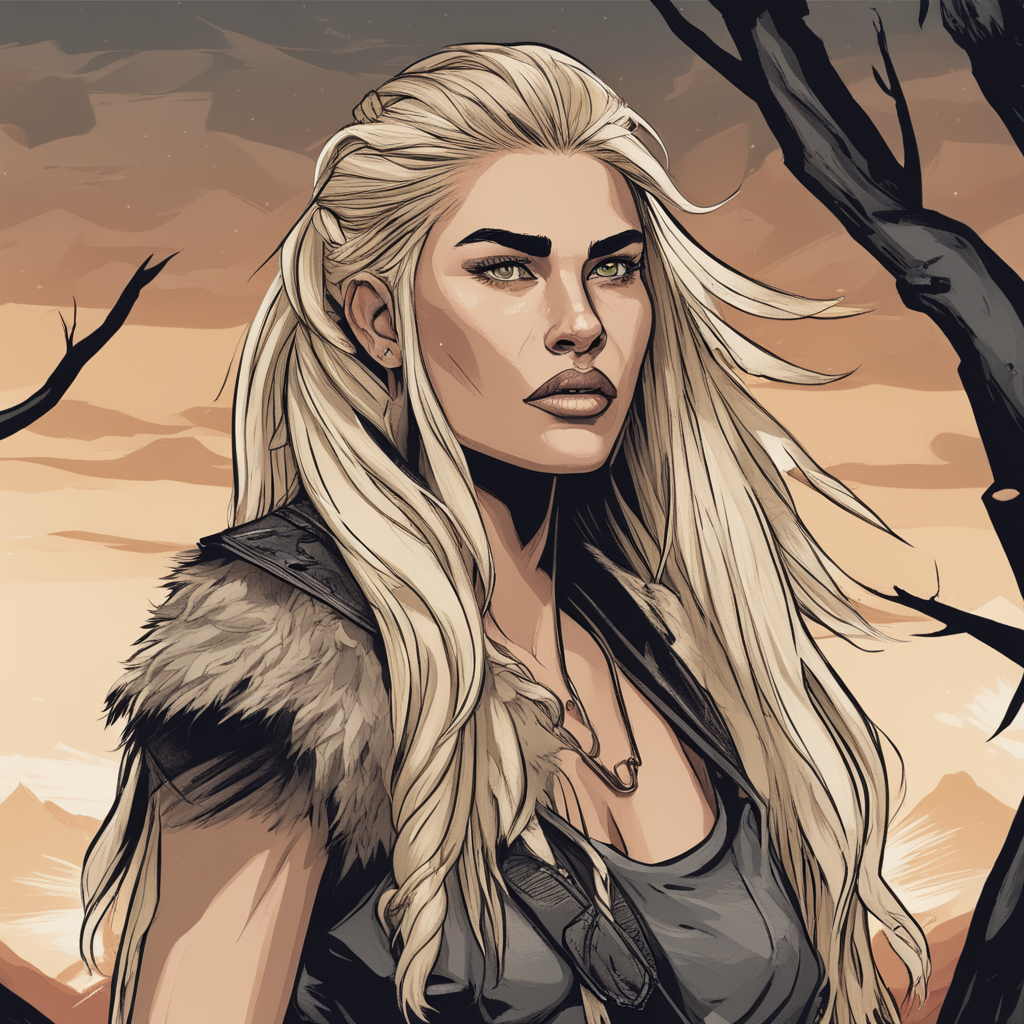
\includegraphics{create-a-digital-illustration-of-branda-a-fierce-and-legendary-woman-with-long-blonde-hair-in-a-hal.png}
\caption{create-a-digital-illustration-of-branda-a-fierce-and-legendary-woman-with-long-blonde-hair-in-a-hal.png}
\end{figure}

Informazioni Generali

Età: 35

Data di nascita: 13/07/1988

Luogo di nascita: Ducatomarrano

Razza: Umana

Classe: Barbara, Via del Totem Guerriero (Lupo della Sila)

Alleati: Gilda dei Guardiani

Nemesi:

Alias: la Fiera


\subsection{Descrizione Generale}\label{descrizione-generale}


\begin{figure}
\centering
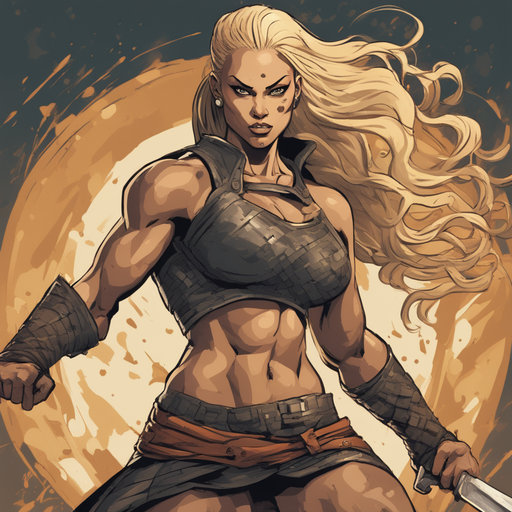
\includegraphics{create-a-digital-illustration-of-branda-a-fierce-and-legendary-woman-with-long-blonde-hair-shaved-o-2.png}
\caption{create-a-digital-illustration-of-branda-a-fierce-and-legendary-woman-with-long-blonde-hair-shaved-o-2.png}
\end{figure}

Branda Gunnarsson, conosciuta come Branda la Fiera, è una figura
leggendaria che si è guadagnata una fama straordinaria Come feroce
avventuriera sempre alla ricerca di avversari più potenti. La sua forza
titanica, la determinazione inarrestabile e l'impegno senza compromessi
nel proteggere la terra l'hanno resa un'icona indiscussa tra gli
avventurieri delle terre selvagge di Valtara.

\subsection{Biografia}\label{biografia}


\subsubsection{Infanzia}\label{infanzia}


Branda la Fiera è nata nel piccolo villaggio di montagna di
Ducatomarrano, circondato da maestose valli e foreste remote. La sua
infanzia è stata segnata da avventure all'aria aperta e da una profonda
connessione con la natura. Fin da piccola, Branda dimostrava una
straordinaria forza fisica e un amore per la vita all'aria aperta. I
suoi genitori, un abile cacciatore e una maestra tessitrice, le hanno
trasmesso preziose abilità di sopravvivenza.

Tuttavia, il destino ha giocato un brutto scherzo quando, all'età di
otto anni, il suo villaggio fu devastato da una terribile inondazione
causata da una violenta tempesta. Questo evento traumatico ha segnato
profondamente Branda e ha risvegliato in lei una determinazione a
proteggere le persone e la natura.

\subsubsection{Adolescenza}\label{adolescenza}


Dopo l'evento dell'inondazione, Branda ha lasciato il suo villaggio
natale in cerca di avventure. Nell'adolescenza, ha viaggiato per
Valtara, esplorando terre sconosciute e affrontando una serie di sfide.
Si è allenata duramente, affinando le sue abilità nel combattimento e
imparando a sopravvivere nelle condizioni più ostili.

Durante questo periodo, ha incontrato e si è alleata con vari
avventurieri, apprendendo da ognuno di loro e guadagnando una
reputazione per il suo coraggio e la sua abilità nel combattimento. Ha
partecipato a missioni per proteggere carovane, sconfiggere mostri e
assistere le comunità in difficoltà.

\subsubsection{Vita Adulta e giorni
nostri}\label{vita-adulta-e-giorni-nostri}


Dopo anni di avventure e crescita personale, Branda ha deciso di
stabilirsi nella pericolosa Foresta dei Giganti in cerca di sfide ancora
più grandi. Questa foresta selvaggia e misteriosa è diventata il suo
nuovo territorio di caccia, dove ha combattuto contro molte delle
creature più feroci e rare del mondo. Qui, ha sviluppato ulteriormente
le sue abilità e ha guadagnato una reputazione tra gli avventurieri come
una forza della natura.

Un giorno, mentre era alla ricerca di un leggendario alce d'argento che
infestava la foresta, ebbe una visione straordinaria di uno spirito lupo
della Sila. Questo incontro divino le rivelò la via della redenzione e
la spinta a mettere le sue abilità al servizio della natura e della
pace. Da allora, Branda ha abbandonato la vita errante per unirsi alla
Gilda dei Guardiani Protettori della Sila e dei Lupi, dedicando la sua
forza e il suo coraggio a proteggere la regione di Valtara e a mantenere
l'ordine tra le creature selvatiche e gli abitanti umani

\subsection{Carriera}\label{carriera}


La carriera di Branda la Fiera è segnata da numerosi combattimenti
eroici e imprese leggendarie. La sua fama come avventuriera la precede,
ed è conosciuta per le sue gesta coraggiose nella Foresta dei Giganti,
dove ha affrontato, da sola, creature temibili come gli orsi delle
caverne giganti, i lupi mannari e si dice persino dei troll.

Dopo la sua conversione alla causa della protezione della natura, Branda
ha continuato a dimostrare la sua dedizione, lavorando con la Gilda dei
Guardiani Protettori della Sila e dei Lupi per preservare gli ecosistemi
di Valtara e mantenere la pace tra le creature selvatiche e gli abitanti
umani. La sua forza, abilità nel combattimento e il suo spirito guida le
hanno permesso di diventare una figura rispettata e una guida per i
giovani aspiranti avventurieri.

\subsection{Personalità}\label{personalituxe0}


Branda è conosciuta per la sua personalità forte e sicura di sé. È prona
all'ira quando è necessario, ma ha imparato a canalizzare la sua rabbia
in modo positivo per combattere le minacce che si presentano. È
appassionata della birra e delle sfide di forza, spesso partecipando a
gare di bevute e gare di sollevamento pesi nei luoghi che visita.

Tuttavia, la sua dedizione alla protezione della natura e la sua
connessione con lo spirito guida del lupo della Sila le conferiscono
anche un lato compassionevole e altruista. È pronta a difendere gli
oppressi e a sacrificare tutto per mantenere l'armonia nella Valtara. La
sua personalità complessa la rende una figura affascinante nel mondo di
D\&D, ammirata sia per la sua forza fisica che per il suo spirito
indomito.


\section{Caravaggio}\label{caravaggio}


\begin{figure}
\centering
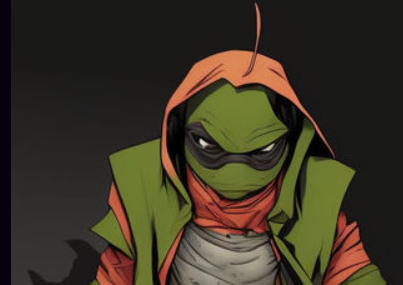
\includegraphics{Screenshot_2023-10-03_204548.png}
\end{figure}

\subsection{Descrizione Generale}\label{descrizione-generale}



Caravaggio è un monaco turtlefolk guerriero. La sua pelle verde scura e
il robusto guscio marrone lo distinguono tra gli altri della sua razza.
Caravaggio è noto per la sua lealtà, il suo coraggio e la sua
determinazione.

\begin{quote}
Citazione {[}location{]}
\end{quote}

\subsection{Biografia}\label{biografia}


Caravaggio è stato adottato da Splinter, un monaco mausefolk, insieme ai
suoi quattro fratelli. Splinter li ha cresciuti e addestrati alle arti
marziali, insegnando loro l'importanza della disciplina e della
protezione degli altri. Durante un viaggio in nave, un tremendo
naufragio ha separato Caravaggio dalla sua famiglia. Ha passato anni a
cercarla, senza mai darsi per vinto, ma non l'ha mai trovata.

\subsection{Carriera}\label{carriera}


Caravaggio ha trovato una nuova casa nelle terre di Valtara, dove ha
messo le sue abilità da combattente a servizio della gilda dei
Protettori. La sua esperienza in combattimento lo ha reso un membro
prezioso dell'organizzazione, impegnato a proteggere la regione dagli
innumerevoli pericoli che la minacciano. Il suo impegno nella gilda è
stato fonte di grande orgoglio, e ha dimostrato di essere un leader
calmo e risoluto quando è necessario.

\subsection{Personalità}\label{personalituxe0}


Caravaggio è noto per la sua lealtà e il suo coraggio. È determinato a
proteggere gli altri dopo aver perso la sua famiglia nel naufragio. Il
principale obiettivo di Caravaggio è riunirsi con i suoi fratelli e con
il suo mentore Splinter. Nel frattempo, si impegna a proteggere Valtara
e le persone che la abitano dai molteplici pericoli che la circondano.
La ricerca dei suoi fratelli è un impegno personale che lo guida in ogni
azione che intraprende.


\section{Disis Iulukinfor}\label{disis-iulukinfor}


\begin{figure}
\centering
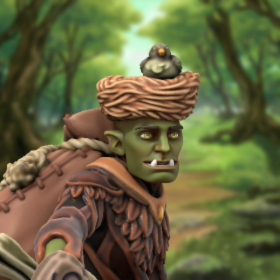
\includegraphics{Disis_Iulukinfor-Token.png}
\caption{Disis Iulukinfor-Token.png}
\end{figure}

Informazioni Generali

Età:

Anno di nascita:

Paese di nascita: Metauros

Razza:

Relazioni:

Alleati:

Nemesi:

Possedimenti importanti:


\subsection{Descrizione Generale}\label{descrizione-generale}


\begin{figure}
\centering
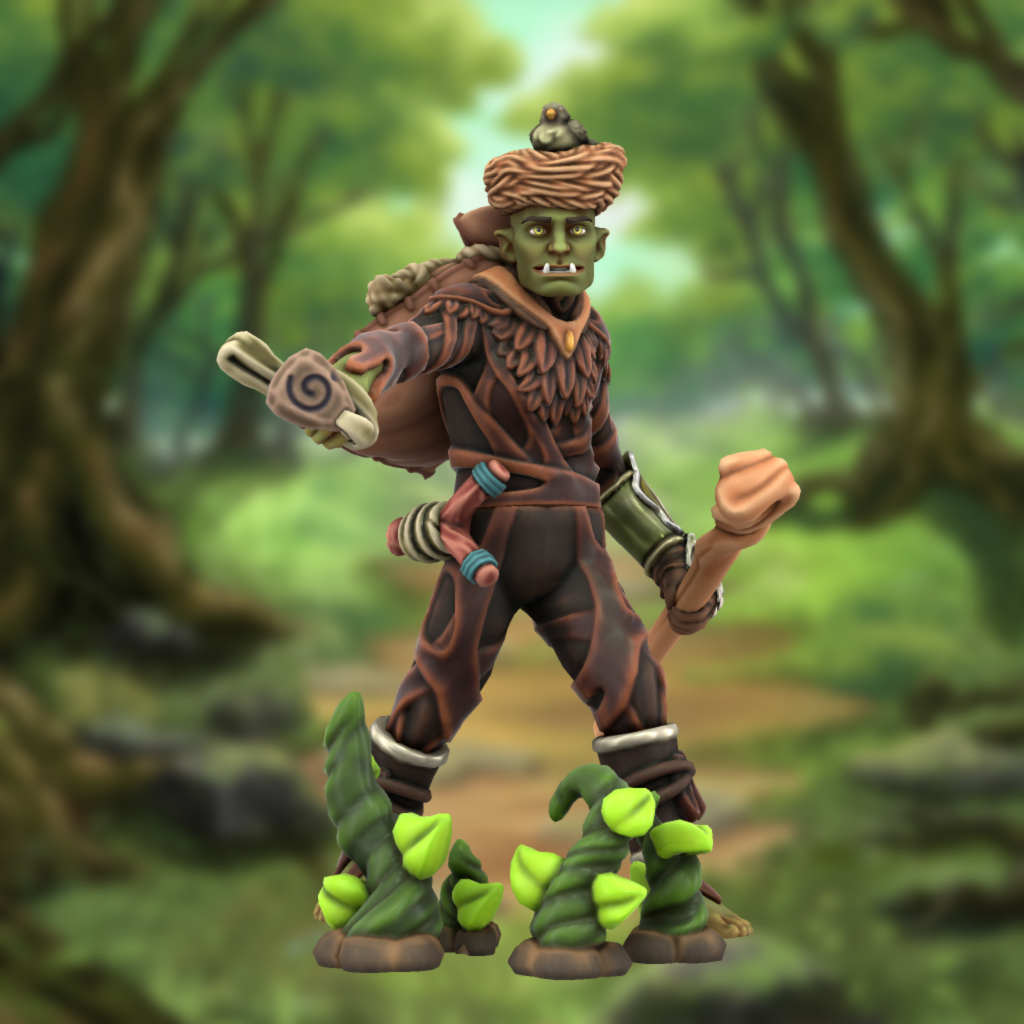
\includegraphics{Disis_Iulukinfor-portrait.png}
\caption{Disis Iulukinfor-portrait.png}
\end{figure}

Disis Iulukinfor è un mezz'orco druido, incarnando l'armonia tra umanità
e natura. La sua pelle abbronzata è attraversata da cicatrici, simboli
del suo passato selvaggio. Gli occhi riflettono saggezza e curiosità,
mentre una chioma corvina incornicia un volto dal fascino unico. Il suo
corpo atletico rivela la profonda connessione con la foresta. Abbigliato
in tonalità terrose, emana un'aura pacifica, trasmettendo sicurezza e un
attaccamento profondo alla natura.

\begin{quote}
``Non sono questi i druidi che state cercando''
\end{quote}

\subsection{Biografia}\label{biografia}


La storia di Disis Iulukinfor inizia con un'origine insolita, nato
dall'incontro tra due mondi, quello umano e quello degli orchi.
Abbandonato poco dopo la nascita nei recessi profondi della foresta,
Disis ebbe la fortuna di essere trovato e adottato dalle creature della
natura. Cresciuto tra animali, spiriti della foresta e creature fatate,
Disis fu avvolto dall'abbraccio amorevole di un ambiente che lo
considerava un proprio figlio. La sua crescita fu segnata
dall'apprendimento dei segreti della natura, dell'arte del druidismo e
della magia che pervadeva gli alberi e le creature stesse. Mentre altri
bambini si familiarizzavano con i confini della società umana, Disis si
immerse nella profonda sapienza delle stagioni, dei venti e degli
animali, diventando un Figlio della Foresta, un protettore e curatore
dell'ambiente che lo aveva accolto. Tuttavia, quando il destino lo portò
a incontrare la civiltà umana, Disis si trovò di fronte a una sfida del
tutto nuova. Confuso e spaesato, si sforzò di adattarsi a usi e costumi
che gli sembravano estranei. La sua capacità di comunicare con gli
animali e il suo cuore gentile gli permisero di stringere amicizie
preziose, aprendo lentamente le porte a un mondo più ampio e complesso.
La sua vita divenne una mescolanza di momenti di contemplazione profonda
nei boschi e di interazioni con le persone che avevano accolto il suo
spirito gentile. Con il tempo, Disis si trasformò in un guardiano della
foresta, un difensore delle creature selvatiche e un portavoce della
natura, cercando di far comprendere agli altri l'importanza di
preservare l'equilibrio dell'ambiente. Liberamente intraprendendo il suo
cammino tra la foresta e le società umane, Disis incarna l'unione di due
mondi e lotta per proteggere l'eredità della foresta che lo ha nutrito,
portando il suo amore per la natura e la sua determinazione a difendere
gli innocenti in ogni angolo del mondo.

\subsection{Carriera}\label{carriera}


La carriera di Disis Iulukinfor non è stata definita da titoli o
posizioni, ma piuttosto da un profondo legame con la natura e il suo
ruolo come guardiano degli equilibri naturali. Fin dalla giovane età,
Disis è stato introdotto alla magia e alla saggezza druidica dalla
foresta stessa. Questa connessione lo ha guidato in un percorso di
apprendimento costante, in cui ha imparato a comunicare con gli animali,
a manipolare le energie naturali e a proteggere l'ambiente circostante.

Inizialmente cresciuto lontano dalla società umana, la sua carriera è
stata forgiata nell'oscurità della foresta, dove ha agito come
intermediario tra le creature selvatiche e gli spiriti della natura. La
sua abilità nel comunicare con gli animali gli ha permesso di sviluppare
un'intesa profonda con le creature che popolano i boschi, facendo di lui
un protettore naturale e un mediatore nei conflitti tra le varie specie.

Con il passare del tempo, il suo ruolo si è espanso, portandolo ad
interagire sempre di più con la società umana. Disis ha iniziato a
condividere la sua conoscenza della natura con coloro che desideravano
ascoltarlo, spiegando l'importanza di rispettare l'ambiente e di
preservare l'equilibrio ecologico. Ha partecipato a iniziative di
conservazione, educando le persone sulle pratiche sostenibili e guidando
escursioni per far conoscere l'ambiente naturale.

La sua carriera non è limitata a un singolo percorso; piuttosto, è un
intreccio di momenti trascorsi nel fitto dei boschi, conversazioni con
creature alate e lezioni impartite su come coesistere in armonia con la
natura. Disis incarna il legame tra l'umanità e il regno naturale,
portando con sé l'eredità del suo passato e la responsabilità del suo
futuro, sempre impegnato a difendere la bellezza e l'equilibrio del
mondo naturale che ama e protegge.

\subsection{Personalità}\label{personalituxe0}


La personalità di Disis Iulukinfor è un intreccio di sfumature,
riflettendo sia l'influenza della natura che la complessità della sua
dualità come mezz'orco. Riservato e riflessivo, Disis porta con sé la
tranquillità dei boschi, un'aura che invita alla contemplazione e al
rispetto. La sua natura tranquilla è un riflesso dell'armonia che cerca
di promuovere nel mondo, facendolo apparire spesso in uno stato di calma
serena.

La sua gentilezza è disarmante, il suo cuore aperto a tutti coloro che
si dimostrano rispettosi e desiderosi di ascoltare le voci della natura.
Con una comunicazione che va al di là delle parole, è in grado di
stabilire connessioni profonde con le creature della foresta, offrendo
amicizia e comprensione dove altri potrebbero vedere solo ferocia.

Sebbene riservato, Disis ha un lato avventuroso e curioso. La sua natura
di Figlio della Foresta lo spinge a esplorare nuovi territori, sia
fisici che emotivi. Questa curiosità lo ha portato a interagire con la
società umana, sfidando le sue ansie e cercando di capire il mondo al di
fuori delle selve.

La sua personalità riflette un profondo rispetto per tutte le forme di
vita. È capace di compassione e di provare dolore per il sofferenza
altrui, ma è altrettanto capace di agire con fermezza quando la natura è
minacciata. La sua determinazione a proteggere l'ambiente naturale e le
creature che vi abitano lo rende un avvocato appassionato per la
conservazione.

In sintesi, Disis è un individuo dalla personalità riflessiva, gentile e
protettiva, ispirato dalla saggezza della natura e determinato a
diffondere armonia e comprensione. La sua personalità è un riflesso del
mondo che abbraccia, un mondo di connessioni profonde e di equilibrio
sottolineato da una passione incrollabile per la conservazione e la
protezione.


\section{Don Tammeo}\label{don-tammeo}


\begin{figure}
\centering
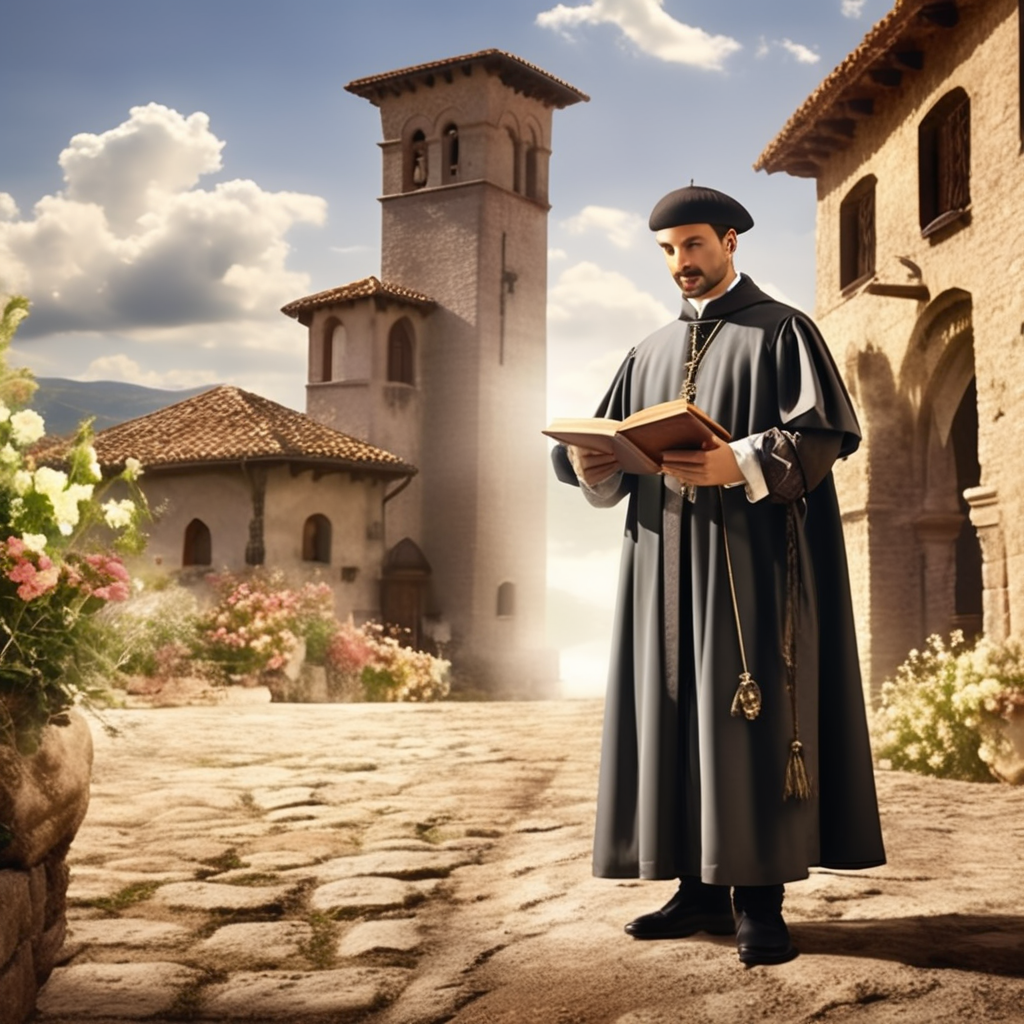
\includegraphics{create-images-of-don-matteo-the-italian-tv-character-in-a-medieval-setting-envision-him-as-a-bene.png}
\end{figure}

\subsection{Descrizione Generale}\label{descrizione-generale}



Don Tammeo è l'incarnazione della speranza nelle strade di Eldrid, un
orfano che ha abbracciato la fede di Luminara Libertas. Membro devoto
della Gilda dei Protettori, la sua presenza irradia compassione e
giustizia, offrendo luce in un mondo avvolto dall'oscurità.

\begin{quote}
``Tutti quanti abbiamo un estremo bisogno di sentirci amati. Ma non c'è
nessuna persona che può colmare questo infinito bisogno d'amore che
abbiamo!'' - Don Tammeo
\end{quote}

\subsection{Biografia}\label{biografia}


\subsubsection{Infanzia}

Don Tammeo è nato sotto il cielo di
\href{Eldrid\%20bd820bb9f6164b39ae6e611a94748518.md}{Eldrid} , ma il
destino gli riservò un percorso diverso. Abbandonato alla sua sorte fin
dalla nascita, Tammeo fu accolto nelle braccia di un orfanotrofio della
città. Crescendo tra i compagni orfani, sviluppò una forza interiore
alimentata dalla necessità di sopravvivere in un mondo spietato.
Tuttavia, durante la sua infanzia, un misterioso evento cambierà il
corso della sua vita. Una notte, mentre osservava il cielo stellato da
una finestra dell'orfanotrofio, ebbe una visione rivelatrice che lo
avvicinò alla fede. Un senso di libertà pervase il suo cuore,
spingendolo a cercare il significato più profondo della vita.

\subsubsection{Adolescenza}

Il richiamo della fede non abbandonò Don Tammeo nemmeno
nell'adolescenza. Spinto dalla visione misteriosa della sua infanzia, si
dedicò agli studi religiosi presso i templi di Eldrid. Con passione e
determinazione, prese i voti e divenne un servo devoto di una divinità
legata al culto della libertà. La sua fede non era solo un insieme di
dogmi, ma una forza guida che plasmò il suo carattere. Tammeo imparò a
condividere il messaggio di speranza e libertà con coloro che
incontrava, diventando una figura di ispirazione per gli altri giovani
che cercavano un significato nella loro esistenza.

\subsubsection{Età Adulta}

Don Tammeo, ora un uomo maturo con il cuore pervaso dalla fede, decise
che la sua missione doveva estendersi oltre le mura del tempio. Sentendo
il richiamo di aiutare coloro che erano in difficoltà, si unì alla Gilda
dei Protettori, un gruppo di individui devoti alla protezione e al
soccorso dei più deboli e bisognosi. La sua dedizione alla giustizia e
la sua connessione con la divinità lo resero un membro rispettato della
gilda. Armato della sua fede incrollabile e della sua compassione per
gli altri, Don Tammeo si adoperò per risolvere i crimini, difendere gli
indifesi e portare la luce della libertà in ogni angolo oscuro di
Eldrid. La sua storia, da orfano a protettore, è diventata una fonte di
ispirazione per la comunità che ha giurato di servire.

\subsection{Carriera}\label{carriera}


Dopo aver preso i voti e aver dedicato la sua vita alla fede di Luminara
Libertas, Don Tammeo ha iniziato il suo cammino come sacerdote
itinerante. Ha viaggiato per Eldrid e le terre circostanti, portando il
messaggio di libertà, speranza e giustizia alle persone che incontrava.
La sua fama di uomo di fede e protettore dei bisognosi ha attirato
l'attenzione della Gilda dei Protettori.

La Gilda, riconoscendo la saggezza e la dedizione di Don Tammeo, lo ha
invitato ad unirsi a loro. Egli ha accettato l'invito, portando la sua
prospettiva unica e il suo zelo per la giustizia all'interno della
gilda. La sua carriera nella Gilda dei Protettori è caratterizzata da
numerosi successi nell'aiutare coloro che sono vittime di ingiustizia e
nell'affrontare minacce criminali.

Don Tammeo ha guadagnato il rispetto dei suoi compagni di gilda e della
comunità di Eldrid, diventando un leader spirituale oltre che un
protettore fisico.

\subsection{Personalità}\label{personalituxe0}


Don Tammeo è un'anima gentile, permeata da una compassione inesauribile.
La sua gentilezza si manifesta attraverso ogni parola e azione, offrendo
conforto a chi è in difficoltà e speranza a coloro che ne hanno bisogno.
La sua fede profonda, ancorata al culto di Luminara Libertas, si traduce
in una determinazione instancabile nel perseguire la libertà e la
giustizia per tutti. Tammeo incarna l'ottimismo, vedendo la luce della
speranza anche nei momenti più bui. La sua integrità morale è come una
guida luminosa, ispirando gli altri a seguire un cammino di rettitudine.
In seno alla Gilda dei Protettori, Don Tammeo assume il ruolo di leader
spirituale, le sue parole fungono da faro guida e il suo impegno per la
causa della libertà crea un legame indissolubile con coloro che
condividono la sua missione. La sua presenza, carica di saggezza e
amore, si staglia come un rifugio sicuro per chi cerca giustizia e
speranza nelle terre di Eldrid


\section{Dorian Be}\label{dorian-be}


\begin{figure}
\centering
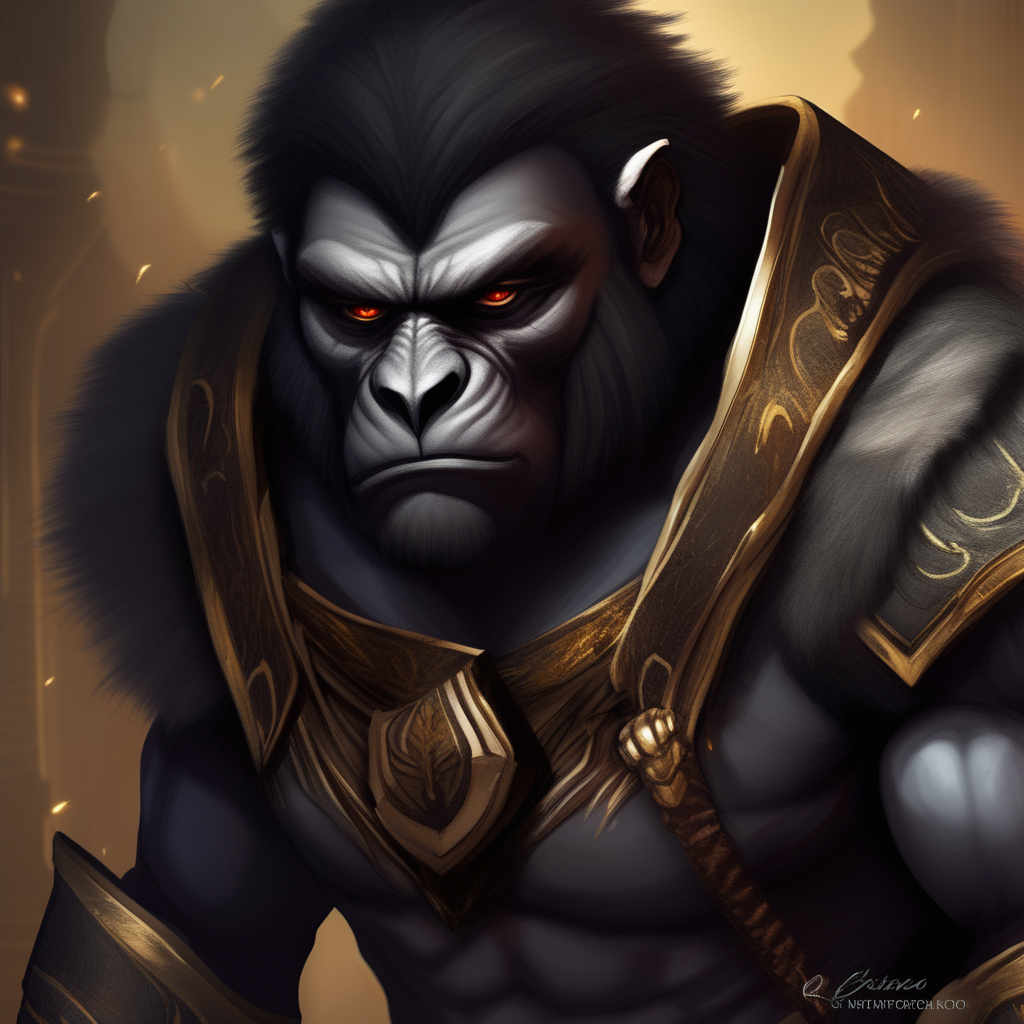
\includegraphics{create-an-image-of-dorian-be-a-heroic-character-from-a-fantasy-world-dorian-is-a-corvilus-a-race---2.png}
\end{figure}

\subsection{Descrizione Generale}\label{descrizione-generale}



Dorian Be è un personaggio di spicco, noto per la sua storia di coraggio
e dedizione nel difendere coloro che sono indifesi. Appartenente alla
misteriosa razza dei Corvilus, che ricorda i gorilla alati, Dorian ha
affrontato tragici eventi che hanno cambiato il corso della sua vita.
Durante la sua carriera circense, condivisa con il suo amato fratello
Haram, ha intrattenuto le folle con spettacoli di giocoleria e abilità
acrobatiche che hanno incantato il pubblico. Tuttavia, una tragedia ha
portato alla perdita delle sue ali e alla morte di Haram, spingendo
Dorian a intraprendere un profondo viaggio di crescita personale. Rinato
come guerriero coraggioso, Dorian ha sviluppato abilità straordinarie
nel combattimento corpo a corpo e la magia arcanica. La sua personalità
compassionevole e protettiva lo ha reso un eroe errante leale, pronto ad
aiutare chiunque abbia bisogno e a portare speranza nei cuori di chi
incontra nel suo cammino.

\begin{quote}
``Tempestate di Like se vi è piaciuta la performance'' - Dorian rivolto
al pubblico
\end{quote}

\subsection{Biografia}\label{biografia}


Dorian Be è nato in un circo itinerante, dove insieme al suo adorato
fratello, Haram Be, intratteneva il pubblico con spettacoli di
giocoleria e abilità acrobatiche. Cresciuto in un ambiente affettuoso e
felice, la loro famiglia circense si considerava una vera e propria
famiglia allargata.

\subsubsection{L'Incidente Tragico}
Un giorno, durante una delle loro esibizioni con bastoni infuocati, un
bambino umano si avventurò inavvertitamente nel perimetro dello
spettacolo. Il fratello di Dorian, Haram, fu distratto dal bambino e
perse il controllo dei bastoni, mettendo in pericolo la vita del
piccolo. Haram, per proteggere il bambino, si lanciò su di lui a
coprirlo, ma fu scambiato per una minaccia e ucciso da una guardia di
paese spaventata.

\subsubsection{La Perdita delle Ali}
Durante la confusione che seguì, Dorian cercò di difendere il corpo
senza vita di Haram, ma fu sopraffatto dalla folla infuriata. Durante la
lotta, subì una profonda ferita sull'ala sinistra da un oggetto
appuntito, rendendo le sue ali irrimediabilmente danneggiate. Incapace
di volare e devastato dalla perdita di suo fratello, Dorian fuggì
portando con sé il corpo del defunto Haram.

\subsubsection{Il Viaggio di Crescita}
Per onorare la memoria di Haram e la loro eredità circense, Dorian
intraprese un lungo viaggio di crescita personale. Cercò maestri saggi e
guerrieri per apprendere le arti del combattimento, della magia e della
forza interiore. Durante il suo viaggio, sviluppò abilità marziali,
apprese a canalizzare l'energia arcana e mantenne vivo il legame con la
natura e le creature alate.

\subsubsection{La Rinascita di Dorian Be}
Dorian Be si trasformò in un combattente agile e coordinato, compensando
la mancanza delle ali con una forza fisica e spirituale incredibile.
Adottò uno stile di vita rispettoso della natura e si impegnò a
proteggere gli esseri vulnerabili, come aveva fatto con il bambino
durante l'incidente che cambiò la sua vita.

\subsubsection{Il Protettore dei Deboli}
Oggi, Dorian Be è noto come un eroe errante, un guerriero
compassionevole che gira il mondo per difendere i deboli, sconfiggere il
male e mantenere vivo lo spirito del circo itinerante che un tempo
condivise con suo fratello Haram. La sua storia toccante e la sua
dedizione nell'assumere la difesa degli oppressi lo hanno reso un
personaggio famoso e rispettato in tutto il mondo di D\&D.

\subsubsection{Eredità di Haram Be}
Dorian Be porta sempre con sé il ricordo del fratello Haram, che
sacrificò la sua vita per proteggere un innocente. Parlando di Haram, i
suoi occhi si illuminano di amore e tristezza, mostrando il legame
indissolubile tra i due fratelli. La memoria di Haram è la forza che
guida Dorian nel suo percorso, e il nome ``Dorian Be'' è diventato un
simbolo di coraggio, protezione e speranza nel mondo di Valtara.

\subsection{Carriera}\label{carriera}


La vita professionale di Dorian può essere divisa in due fasi: la vita
da circense e la vita da guerriero

\subsubsection{Carriera Circense}\label{carriera-circense}

La carriera circense di Dorian Be è iniziata fin da quando era un
giovane gorilla alato. Cresciuto nel cuore di un circo itinerante, ha
imparato sin da piccolo le abilità acrobatiche, la giocoleria e il
carisma necessari per intrattenere il pubblico. Sotto la guida amorevole
dei suoi genitori adottivi e di suo fratello Haram, Dorian si è
trasformato in un abile artista circense, catturando l'attenzione delle
folle con la sua presenza carismatica e le sue abilità impressionanti.
Il duo di fratelli, Dorian e Haram, era la stella del circo, attirando
sempre il pubblico più numeroso. Le loro esibizioni erano spettacolari e
coinvolgenti, con acrobazie mozzafiato e numeri di giocoleria che
sembravano sfidare la gravità stessa. Il legame fraterno tra Dorian e
Haram era evidente sul palco, trasmettendo calore e amore agli
spettatori, che si sentivano parte di una grande famiglia circense.
L'incidente tragico che portò alla morte di Haram e alla perdita delle
ali di Dorian segnò la fine della sua carriera circense. Il circo,
devastato dalla tragedia, continuò senza di loro, ma Dorian sentì di non
poter più esibirsi senza suo fratello. Decise di intraprendere un nuovo
cammino, cercando di onorare la memoria di Haram in altri modi e di
trovare un nuovo scopo nella sua vita.

\subsubsection{Carriera da Guerriero}\label{carriera-da-guerriero}

Dopo aver vissuto un periodo di lutto e riflessione, Dorian Be iniziò il
suo viaggio di crescita personale, intraprendendo una nuova carriera
come guerriero. Sentiva di avere una responsabilità nei confronti della
sua famiglia circense e del ricordo di suo fratello. Decise che doveva
migliorarsi e diventare più forte per poter proteggere coloro che amava
e per difendere gli indifesi da eventuali pericoli. Durante il suo
viaggio, Dorian cercò insegnanti e mentori in diverse arti di
combattimento e magia. Studiò con maestri di arti marziali, imparando a
padroneggiare diverse tecniche di combattimento corpo a corpo. Inoltre,
sviluppò la sua abilità nella magia, scoprendo di poter canalizzare
l'energia arcanica e lanciare incantesimi per difendersi e aiutare gli
altri. Con determinazione e costanza, Dorian affinò le sue abilità,
combinando la forza fisica con la saggezza e la magia. Integrandole con
l'agilità acquisita nella sua carriera circense, Dorian divenne un
guerriero straordinario, capace di fronteggiare nemici e proteggere gli
innocenti. La sua connessione con la natura e le creature alate gli
conferì un legame speciale con gli animali, che spesso lo aiutano nelle
sue missioni. Ha sviluppato una particolare affinità con gli uccelli,
che considera i suoi messaggeri e compagni nell'avventura. Questo legame
speciale gli ha permesso di sviluppare uno stile di combattimento unico,
prendendo ispirazione dai movimenti aggraziati degli uccelli in volo.
Oggi, Dorian Be è un eroe errante, un combattente leale e
compassionevole, con l'abilità di proteggere gli altri con la sua forza
fisica e la magia, mentre mantiene sempre vivo lo spirito del circo
itinerante che una volta condivideva con suo fratello. La sua carriera
da guerriero è diventata una fonte di ispirazione per molti, un esempio
di come il coraggio e la dedizione possano trasformare una tragedia in
un segno di speranza e di difesa per chiunque abbia bisogno di aiuto.

\subsection{Personalità}\label{personalituxe0}


Dorian Be possiede una personalità profondamente empatica e
compassionevole, che è stata plasmata dalle tragedie che ha vissuto. La
perdita di suo fratello Haram ha lasciato un segno indelebile nel suo
cuore, trasformandolo in un individuo protettivo e devoto a coloro che
hanno bisogno di aiuto. È un'anima gentile, sempre pronta a tendere una
mano amica a chiunque sia in difficoltà. Nonostante la sua natura
sensibile, Dorian è anche un individuo coraggioso e tenace. Ha
affrontato numerose sfide e difficoltà nel suo viaggio di crescita,
dimostrando una determinazione inarrestabile nel superarle. La sua
dedizione nel migliorarsi costantemente, sia fisicamente che
mentalmente, lo ha reso un combattente straordinario e un alleato fidato
nei momenti di bisogno. La sua esperienza di circo gli ha donato un
senso dell'umorismo e un lato giocoso, che emergono soprattutto quando è
in compagnia di nuovi amici o quando si trova in situazioni rilassate.
Dorian è sempre pronto a intrattenere il suo gruppo con piccoli trucchi
e acrobazie, portando un po' di leggerezza e divertimento nei momenti
più cupi. Tuttavia, anche se può essere socievole e affabile, Dorian ha
anche dei momenti di intimità e riflessione. I ricordi di suo fratello
Haram possono renderlo triste o nostalgico, ma trova nella sua memoria
la forza per continuare a proteggere e difendere gli altri. La sua
connessione con la natura e le creature alate gli conferisce un profondo
rispetto per l'ambiente circostante e tutte le forme di vita. È un
ambientalista appassionato e cerca sempre di minimizzare l'impatto
negativo che può avere sull'ecosistema, prendendosi cura della fauna e
della flora che lo circondano. Dorian è anche un ascoltatore empatico,
disponibile a dare consigli o conforto quando necessario. Ha imparato
che il potere di proteggere gli altri non si limita solo alla forza
fisica, ma anche a fornire un ascolto attento e un sostegno morale.
Questo atteggiamento compassionevole gli ha guadagnato molte amicizie e
gli ha permesso di formare legami profondi con coloro che incontra nel
suo cammino.


\section{Durso}\label{durso}


\begin{figure}
\centering

\includegraphics{Durso.png}
\caption{Durso.png}
\end{figure}

Informazioni Generali

Età:

Anno di nascita:

Paese di nascita:

Razza: Mezzorco

Relazioni:

Alleati:

Nemesi:

Possedimenti importanti:


\subsection{Descrizione Generale}\label{descrizione-generale}


\begin{figure}
\centering
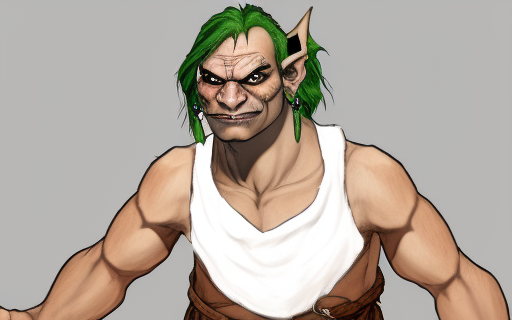
\includegraphics{a-fantasy-orc-that-looks-like-a-male-version-of-barbara-durso-.png}
\caption{a-fantasy-orc-that-looks-like-a-male-version-of-barbara-durso-.png}
\end{figure}

Durso è cresciuto in una tribù di orchi nel cuore della giungla. Fin da
piccolo, si è distinto per la sua stazza imponente e la sua forza
sovrumana. Nonostante l'aspetto minaccioso della sua razza, Durso ha
sempre avuto un cuore buono e un'innata propensione per aiutare gli
altri. Questo lo ha portato spesso a conflitti con gli altri membri
della tribù, che lo consideravano troppo morbido e indulgente.

Un giorno, durante una battuta di caccia, Durso e alcuni compagni della
tribù hanno incontrato un gruppo di avventurieri umani. Durso ha subito
trovato un'affinità con questi stranieri, che non lo giudicavano in base
alla sua razza. Ha iniziato a passare sempre più tempo con loro,
imparando il loro linguaggio e le loro usanze. L'usanza preferita di
Durso era quella nota come ``Postmeridiem V'', secondo la quale tutti si
sedevano attorno ad un fuoco a discutere in maniera semi-seria sui fatti
di cronaca del villaggio.

Con il tempo, Durso ha capito che il suo posto non era nella tribù degli
orchi, ma tra gli avventurieri. Ha lasciato la giungla e si è unito al
gruppo umano, diventando un ciarlatano e uno scaramantico. A volte fa
anche dei riti strani contro la sfortuna, credendo che possano aiutarlo
ad avere successo nelle sue imprese.

La collana di peperoncini che indossa al collo è un talismano che ha
ricevuto da un vecchio sciamano della sua tribù, che gli ha detto che
avrebbe portato fortuna. Durso la porta sempre con sé, convinto che sia
stata la chiave del suo successo come avventuriero.

Nostante la sua parlata un po' rozza, Durso ha un lato più profondo e
riflessivo. Ogni tanto, quando il gruppo si ferma per riposare dopo una
dura avventura, Durso comincia a filosofeggiare e a fare discorsi che
sorprendono i suoi compagni. Proprio come Barbara d'Urso, Durso ha la
capacità di trasformare temi apparentemente banali in riflessioni più
profonde sulla vita e sull'umanità. Anche se a volte i suoi discorsi
possono sembrare un po' strani, i suoi compagni lo rispettano per la sua
saggezza e la sua capacità di vedere le cose da diverse prospettive.

Durso è un buon compagno di squadra e un difensore appassionato dei più
deboli. Anche se non sempre segue le regole, la sua natura caotica buona
lo porta a fare sempre la cosa giusta.

\begin{quote}
``Lei mi sta dicendo che?''
\end{quote}

\subsection{Biografia}\label{biografia}


\begin{figure}
\centering
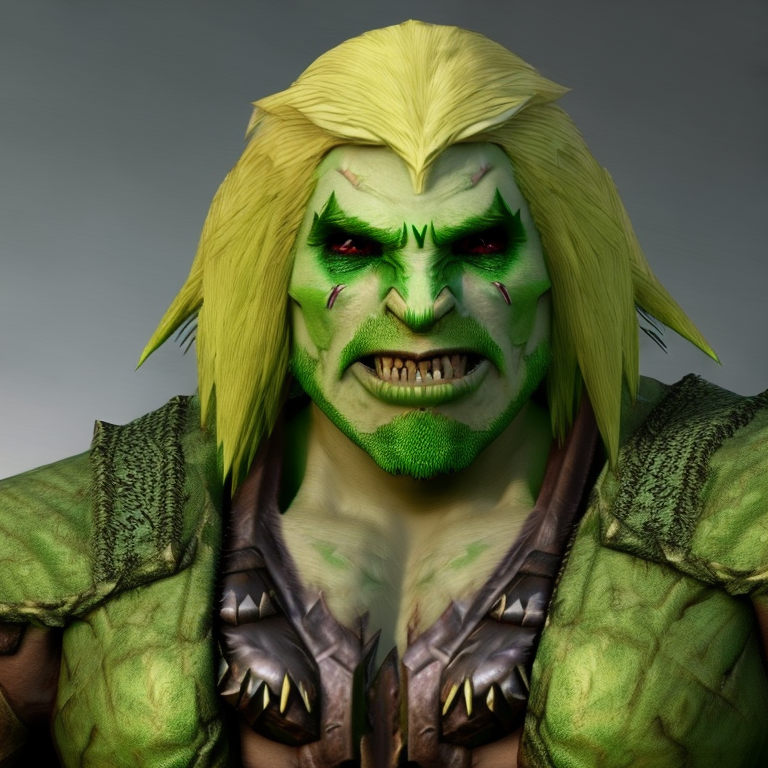
\includegraphics{a-fantasy-orc-that-looks-like-a-male-version-of-barbara-durso-green-skin-blonde-hair--.png}
\caption{a-fantasy-orc-that-looks-like-a-male-version-of-barbara-durso-green-skin-blonde-hair--.png}
\end{figure}

The {[}people group{]} were the region's sole residents prior to the
{[}historical event{]}. {[}New people group{]} arrived in the region
around {[}year{]}.

\subsection{Carriera}\label{carriera}


The history and economic growth of {[}location{]} is tied to
{[}geographic feature{]} which is {[}location's{]} defining
characteristic.

\subsection{Personalità}\label{personalituxe0}



\section{Fabritius Quaterocula (WIP)}\label{fabritius-quaterocula-wip}
\section{Fabritius Quaterocula}\label{fabritius-quaterocula}


\begin{figure}
\centering

\includegraphics{No-Photo-Available-591x591-2.jpg}
\caption{No-Photo-Available-591x591-2.jpg}
\end{figure}

Informazioni Generali

Età: 55

Data di nascita: 9 Maggio 1968

Luogo di nascita: sconosciuto

Razza: Umano

Classe: Guerriero

Alleati:

Nemesi:

Alias:

Professione: Mercenario


\subsection{Descrizione Generale}\label{descrizione-generale}


\begin{figure}
\centering
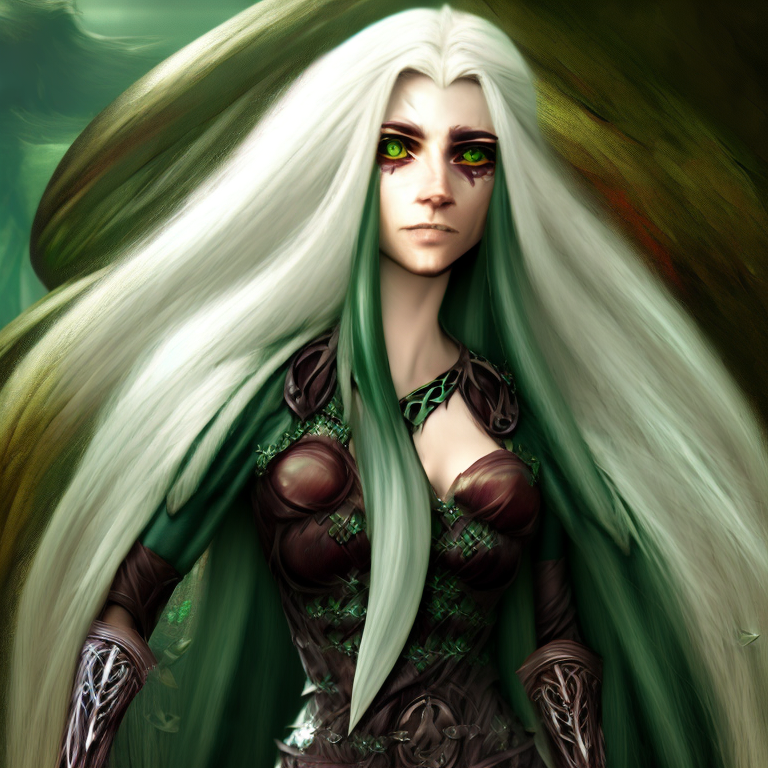
\includegraphics{full-body-portrait-of-a-beautiful-female-elf-with-long-silver-hairs-and-deep-green-eyes-fantasy-se-.png}
\caption{full-body-portrait-of-a-beautiful-female-elf-with-long-silver-hairs-and-deep-green-eyes-fantasy-se-.png}
\end{figure}

Fabritius Quaterocula, conosciuto semplicemente come Fabritius tra gli
ambienti mercenari, è una figura enigmatica e spietata. La sua
reputazione di guerriero senza scrupoli è amplificata dalla sua mancanza
di radici e di un passato noto. La sua avidità è leggendaria, e non
esita a compiere qualsiasi azione, a patto che il prezzo sia adeguato.

\begin{quote}
``Vi faccio vedere come muore un Valtariano'' - Tipico inno di battaglia
di Fabritius
\end{quote}

\subsection{Biografia}\label{biografia}


La vita di Fabritius è avvolta da un velo di mistero. Non ha ricordi
della sua terra natale, né delle sue origini familiari. La sua storia è
una serie di contratti stipulati e denaro guadagnato, senza alcun legame
emotivo che lo lega a un luogo o a una persona. Le storie su di lui sono
spesso accompagnate da sussurri e leggende, alcune delle quali affermano
che abbia venduto la sua anima al diavolo per ottenere il suo spietato
talento bellico, mentre altre sostengono che abbia accumulato così tante
ricchezze da poter comprare qualsiasi cosa, tranne la sua vera identità.

\subsection{Carriera}\label{carriera}


Cresciuto nella scuola della guerra, Fabritius è un maestro di tutte le
armi, un esperto tattico e un assassino spietato quando la situazione lo
richiede. La sua abilità lo rende una presenza temibile e imprevedibile
nei campi di battaglia e tra le ombre delle città. È noto per non fare
domande ai suoi datori di lavoro o sulle loro cause; il suo unico
interesse è il compenso, e ogni contratto rappresenta un'opportunità per
accumulare ulteriori ricchezze. La mancanza di radici e il suo spirito
mercenario fanno sì che Fabritius non conosca alcuna lealtà se non a se
stesso e al suo portafoglio.

\subsection{Personalità}\label{personalituxe0}


Fabritius è un individuo freddo e calcolatore, il cui comportamento è
guidato unicamente dall'avidità e dalla sete di profitto. Nonostante la
sua spietatezza in battaglia, è noto per mantenere un autocontrollo
impeccabile, valutando con attenzione le opportunità che si presentano
per accumulare ricchezza. Non fa domande ai suoi datori di lavoro e
segue gli ordini senza esitazione, a patto che il compenso sia
all'altezza delle sue aspettative.

La sua mancanza di legami emotivi o di un senso di appartenenza a una
comunità lo rende un individuo solitario e privo di scrupoli. Non si fa
scrupoli nel compiere azioni immorali se ciò gli consente di guadagnare
ulteriori monete d'oro. La sua reputazione di individuo imprevedibile e
disposto a tutto per il denaro lo circonda di una sorta di aura di
pericolo.

Fabritius è un individuo isolato, incapace di stabilire relazioni
significative o di instaurare amicizie durature. La sua lealtà è
esclusivamente a se stesso e al suo portafoglio. La sua personalità è
caratterizzata da un pragmatismo senza scrupoli, facendolo agire come un
predatore alla ricerca costante di opportunità per accumulare ricchezze,
indipendentemente dalle conseguenze per gli altri.

\subsection{Coinvolgimenti in Eventi
Recenti}\label{coinvolgimenti-in-eventi-recenti}


\href{Untitled\%20Database\%20cce7df74e0604fb88db6fb1d13af3934.csv}{Untitled
Database}


\section{Gario Miordano}\label{gario-miordano}
\section{Gario Miordano}\label{gario-miordano-1}


\begin{figure}
\centering
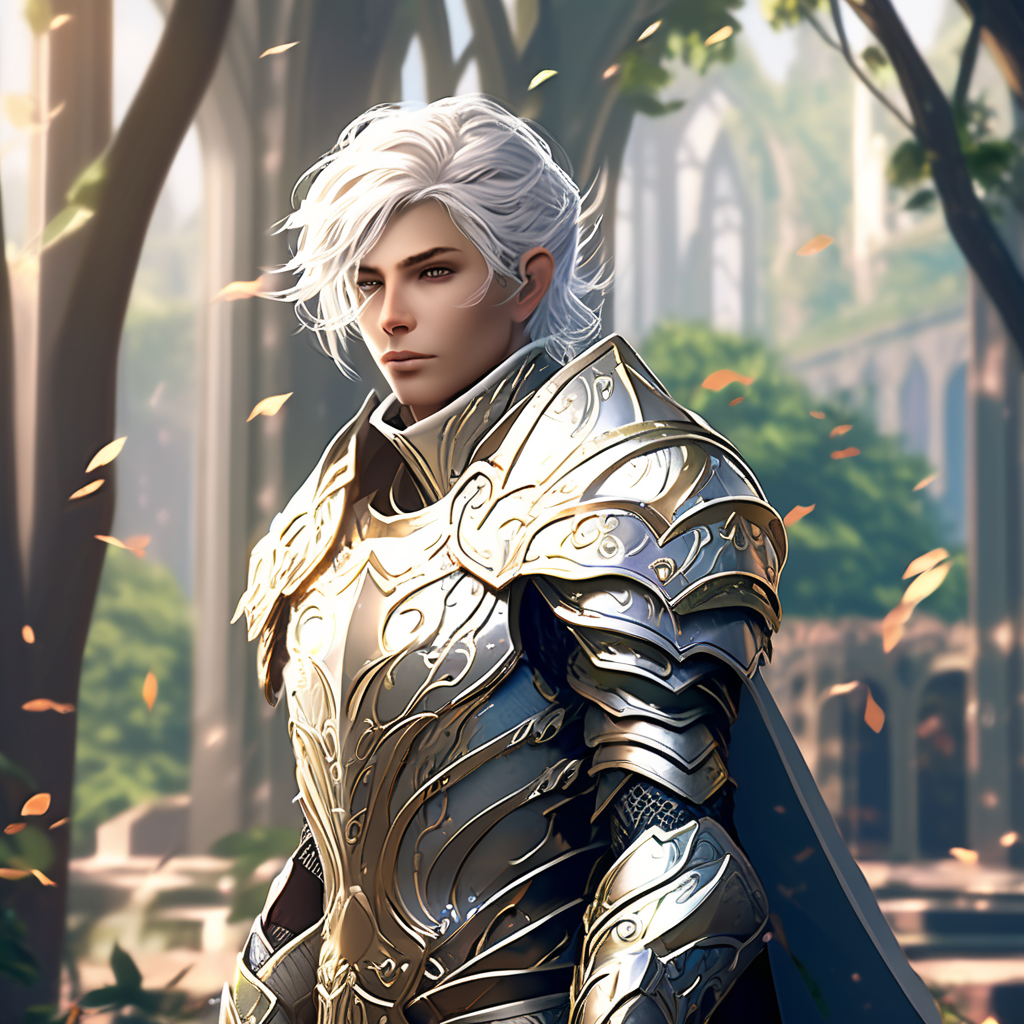
\includegraphics{depict-an-elf-paladin-he-is-a-young-adult-with-short-white-hairs-wearing-full-plate-armour.png}
\caption{depict-an-elf-paladin-he-is-a-young-adult-with-short-white-hairs-wearing-full-plate-armour.png}
\end{figure}

Informazioni Generali

Età: 623

Data di nascita:

Luogo di nascita: Fredo Flu

Razza: Elfo

Classe: Paladino

Alleati:

Nemesi: Le Zucche

Alias:

Professione:


\subsection{Descrizione Generale}\label{descrizione-generale}


\begin{figure}
\centering
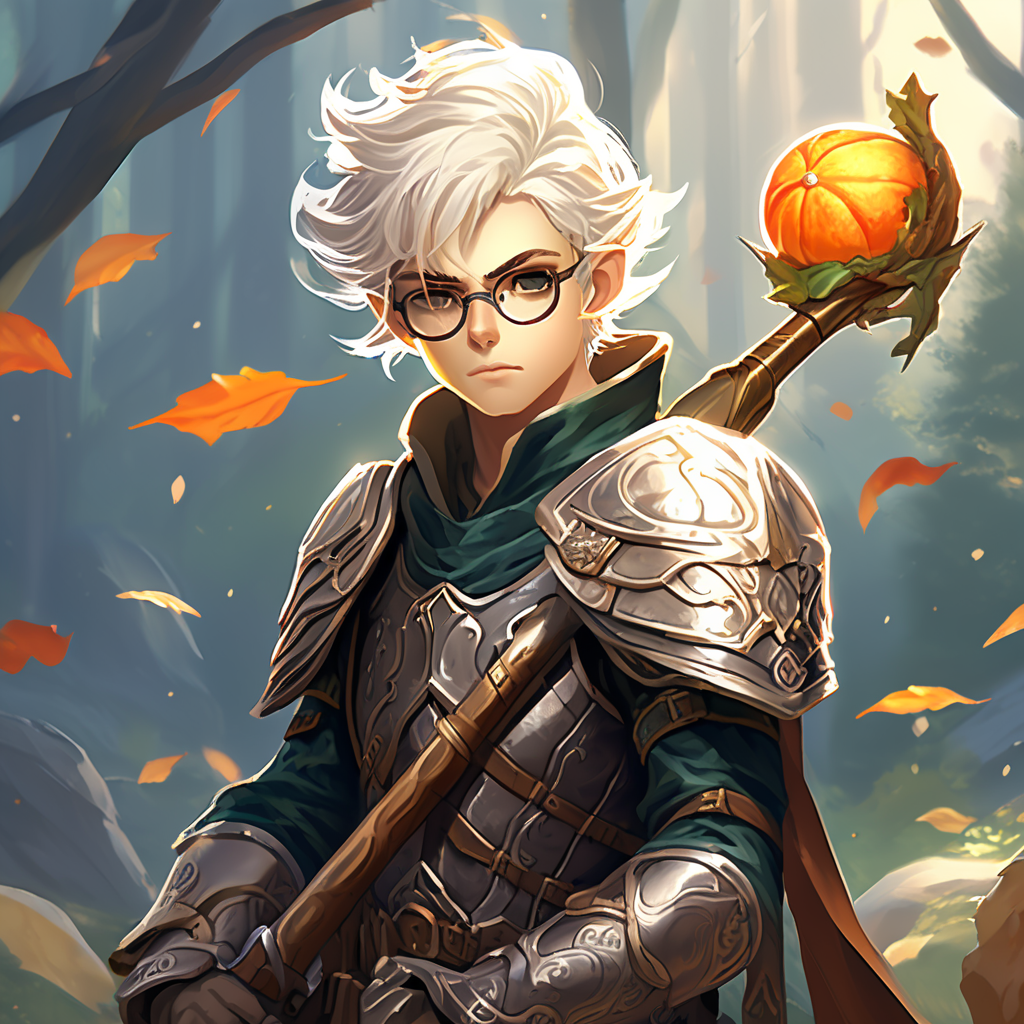
\includegraphics{depict-an-elf-paladin-he-is-a-young-adult-with-short-white-hairs-wearing-full-plate-armour-and-spe-923031639.png}
\caption{depict-an-elf-paladin-he-is-a-young-adult-with-short-white-hairs-wearing-full-plate-armour-and-spe-923031639.png}
\end{figure}

Gario è un elfo paladino di Fredo Flu, con una personalità complessa.
Sebbene animato da un senso di giustizia, è bigotto, xenofobo e
ipocrita, credendo di agire per il bene supremo. Dietro la durezza, ha
un cuore compassionevole, ma le sue azioni spesso suscitano polemiche.

\begin{quote}
``Io le feste di autunno non le voglio festeggiare'' - Gario Miordano
\end{quote}

\subsection{Biografia}\label{biografia}


\subsubsection{\texorpdfstring{\textbf{Origini Nobili e Caduta di
Fredo
Flu}}{Origini Nobili e Caduta di Fredo Flu}}\label{origini-nobili-e-caduta-di-fredo-flu}

Gario Miordano è nato all'interno di una delle più illustri famiglie
elfiche di Fredo Flu, un tempo una delle città più fiorenti e prosperose
del regno elfico. Cresciuto tra l'agio e il lusso, Gario ha goduto di
una vita privilegiata fin dalla sua infanzia, circondato dall'amore e
dall'attenzione della sua famiglia. Tuttavia, la sua vita idilliaca è
stata sconvolta quando una terribile maledizione ha colpito la famiglia
reale di Fredo Flu, causando la sua disfatta e il declino della città.

\subsubsection{\texorpdfstring{\textbf{Fuga a Pandosia e
Coinvolgimento
Politico}}{Fuga a Pandosia e Coinvolgimento Politico}}\label{fuga-a-pandosia-e-coinvolgimento-politico}

Costretto a fuggire insieme alla sua famiglia per sfuggire al destino
che stava per abbattersi su di loro, Gario ha trovato rifugio nella
città di Pandosia, dove è stato accolto da uno dei signori locali.
Durante la sua adolescenza a Pandosia, Gario si è trovato immerso in un
mondo di politica e intrighi, affascinato dalla complessità del potere e
delle relazioni sociali. La sua ambizione lo ha spinto ad avvicinarsi
sempre di più alla scena politica della città, fino a quando non ha
deciso di candidarsi a sindaco.

\subsubsection{\texorpdfstring{\textbf{La Sconfitta e la Profonda
Depressione}}{La Sconfitta e la Profonda Depressione}}\label{la-sconfitta-e-la-profonda-depressione}

Tuttavia, la sua candidatura è stata un fallimento e Gario è stato
sopraffatto da una profonda depressione, incapace di accettare la
sconfitta e il fallimento dei suoi sogni. In preda alla disperazione, ha
abbandonato Pandosia e ha iniziato un lungo viaggio attraverso terre
sconosciute, vagando senza meta per circa cinquant'anni.

\subsubsection{\texorpdfstring{\textbf{Il Giuramento e la Rinascita
Come
Paladino}}{Il Giuramento e la Rinascita Come Paladino}}\label{il-giuramento-e-la-rinascita-come-paladino}

Sulla soglia dei cinquecento anni di età, Gario è giunto in un antico
monastero nascosto tra le montagne, dove ha trovato rifugio e
consolazione. Qui, immerso nella solitudine e nella contemplazione, ha
trovato la fede e ha deciso di prestare giuramento come paladino,
dedicando la sua vita al servizio degli altri e alla difesa dei deboli e
degli oppressi.

\subsubsection{\texorpdfstring{\textbf{La Leggenda dello
Spaccazzucca}}{La Leggenda dello Spaccazzucca}}\label{la-leggenda-dello-spaccazzucca}

Durante i suoi vagabondaggi, Gario si trovò ad affrontare una minaccia
inaspettata: una banda di briganti malvagi che aveva preso d'assalto un
villaggio agricolo. Questi briganti, noti per la loro crudeltà, avevano
preso il controllo del villaggio e avevano iniziato a saccheggiare le
colture di zucche, essenziali per la sopravvivenza della comunità.
Gario, mosso dalla compassione per gli abitanti del villaggio e
determinato a porre fine alla tirannia dei briganti, affrontò i
malviventi con coraggio e astuzia.

Durante la battaglia che ne seguì, Gario afferrò una grande mazza di
legno e la usò con grande maestria contro i suoi avversari. Con ogni
colpo, le zucche che i briganti avevano rubato dal villaggio si
frantumavano sotto la forza travolgente della mazza di Gario. Il suono
sordo degli schianti delle zucche riempiva l'aria mentre Gario
combatteva con ferocia e determinazione. Alla fine, grazie alla sua
abilità nel combattimento e alla sua astuzia, Gario riuscì a sconfiggere
i briganti e a restituire la pace e la sicurezza al villaggio. Da quel
giorno in poi, Gario fu conosciuto come ``Lo Spaccazzucca'', in onore
della sua impresa eroica che aveva visto le zucche rotolare sotto la sua
mazza come se fossero state fatte di vetro.

\subsection{Carriera}\label{carriera}


\subsubsection{Carriera Politica}\label{carriera-politica}

Durante il periodo trascorso a Pandosia, Gario Miordano si immerse
attivamente nella politica locale, attratto dalla complessità dei giochi
di potere e dalle dinamiche sociali della città. Pur non essendo ancora
direttamente coinvolto nella politica ufficiale, Gario partecipò
attivamente alle discussioni comunitarie e alle riunioni pubbliche,
esprimendo le sue opinioni su questioni di interesse cittadino e
sostenendo cause che riteneva giuste e importanti. La sua voce risuonava
con autorità e rispetto tra i suoi concittadini, che apprezzavano la sua
sincerità e la sua dedizione alla causa del bene comune. Questa
esperienza lo ha preparato per la sua futura carriera politica,
fornendogli le basi necessarie per affrontare le sfide e le
responsabilità che avrebbe incontrato nel corso della sua vita pubblica.

\subsubsection{\texorpdfstring{\textbf{Carriera Come
Paladino}}{Carriera Come Paladino}}\label{carriera-come-paladino}

Dopo aver giurato fedeltà al monastero e aver abbracciato la vita da
paladino, Gario Miordano ha dedicato ogni istante della sua esistenza
alla difesa dei deboli e alla lotta contro le forze del male. Grazie
alla sua abilità nel combattimento e alla sua fede incrollabile, ha
affrontato numerosi nemici, da orde di creature oscure a potenti maghi
oscuri, dimostrando sempre una straordinaria determinazione e coraggio.
La sua reputazione di paladino valoroso e intraprendente si è diffusa
rapidamente, guadagnandogli il rispetto e l'ammirazione di coloro che
hanno avuto la fortuna di combattere al suo fianco. Attraverso le sue
imprese eroiche e il suo impegno costante per la giustizia e la
rettitudine, Gario continua a incarnare gli ideali dei Protettori,
servendo come esempio luminoso di sacrificio e dedizione per tutti
coloro che lo incontrano.

\subsection{Personalità}\label{personalituxe0}


Gario Miordano è caratterizzato da un atteggiamento bigotto, xenofobo e
ipocrita, sebbene sia convinto di agire per il bene supremo. La sua
rigida interpretazione delle sue credenze e la sua mancanza di
tolleranza nei confronti di chi è diverso da lui lo portano spesso a
manifestare pregiudizi e discriminazioni verso altre razze e culture.
Pur professando di difendere gli ideali di giustizia e moralità, Gario
mostra spesso un duplice standard nel trattare gli altri, giudicando
severamente i peccati altrui mentre giustifica i suoi stessi
comportamenti discutibili. La sua ipocrisia emerge quando, nonostante le
sue azioni discriminatorie, crede fermamente di essere dalla parte della
rettitudine e della verità. In certi momenti, Gario può dimostrare
generosità e compassione, ma spesso queste qualità sono riservate solo a
coloro che condividono le sue stesse convinzioni, mentre gli altri
vengono trattati con disprezzo e ostilità. In definitiva, la personalità
di Gario Miordano è contraddistinta da una complessa intersezione di
bigottismo, xenofobia e ipocrisia, che lo rende un individuo controverso
e difficile da comprendere.


\section{Gnomio Cartonio}\label{gnomio-cartonio}


\begin{figure}
\centering
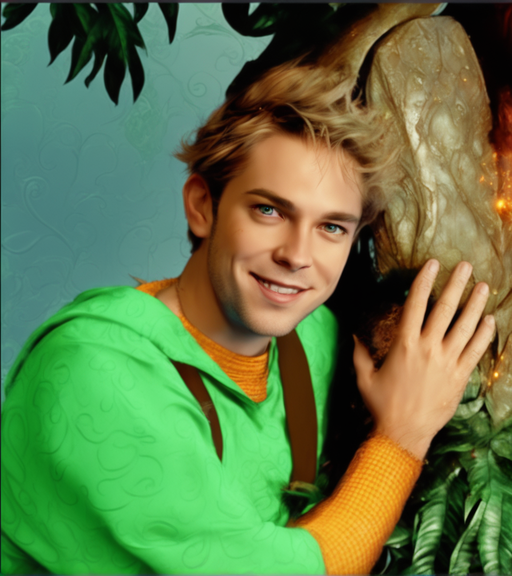
\includegraphics{gnomo-epic-royal-background-big-royal-uncropped-crown-royal-jewelry-robotic-nature-full-shot-.png}
\end{figure}

\subsection{Descrizione Generale}\label{descrizione-generale}



Gnomio è uno gnomo giovane e intraprendente che vive nel tranquillo
Fantabosco, un affascinante villaggio gnomico situato nella Valtara
Meridionale, al confine con il Regno degli Alisei. Sin da bambino, ha
sognato di diventare uno dei più grandi eroi di Fantabosco e ha un
desiderio ardente: uccidere un drago e creare un'armatura di scaglie di
drago che diventi leggendaria a Valtara. La sua vita è un'avventura in
continua evoluzione, guidata dalla passione per la storia dei draghi e
il desiderio di gloria.

\begin{quote}
``Che testa di pigna che sono!''
\end{quote}

\subsection{Biografia}\label{biografia}


Gnomio è nato a Fantabosco da una famiglia di gnomi con una lunga
tradizione di artigianato. Fin dall'infanzia, è stato affascinato dalle
storie dei draghi raccontate dai viaggiatori che passavano per il suo
villaggio. La madre di Gnomio, Mamma Antelitteram, è stata una figura
determinante nella sua vita, spingendolo ad avvicinarsi alla Gilda dei
Protettori per poter garantire il suo sostentamento. Questo è stato un
passo cruciale che ha influenzato la sua carriera.

\subsection{Carriera}\label{carriera}


La passione di Gnomio per la storia dei draghi lo ha spinto a diventare
un abile archeologo, dedicando innumerevoli ore a scavare tra le rovine
antiche e a esaminare manufatti per apprendere tutto ciò che poteva. Da
adulto, ha deciso di diventare un ranger specializzato nella caccia alle
creature magiche, in particolare ai draghi. Ha perfezionato le sue
abilità di combattimento, apprendendo a sopravvivere nella natura
selvaggia e ad affrontare i pericoli della Foresta dei Giganti.

Il suo percorso lo ha portato a viaggiare in luoghi remoti alla ricerca
di indizi sulle possibili dimore dei draghi. L'affiliazione alla Gilda
dei Protettori è stata inizialmente una scelta dettata dalla necessità
finanziaria, ma ha presto compreso che questa opportunità gli avrebbe
permesso di perseguire la sua passione in modo più completo.

\subsection{Personalità}\label{personalituxe0}


Gnomio è noto per la sua determinazione e la sua curiosità insaziabile.
È un individuo tenace, sempre in cerca di nuove conoscenze e disposto a
mettere alla prova se stesso per raggiungere i suoi obiettivi. Tuttavia,
è anche affettuoso e legato alla sua amata Fata Ficarella, che lo ispira
costantemente e gli dà la motivazione per cercare la gloria.

Porta sempre con sé una fiaschetta di cuoio contenente la Scivolizia,
una bevanda tipica del suo villaggio. Questa bevanda particolare è un
segno tangibile delle sue radici e delle sue origini a Fantabosco, ed è
un ricordo costante della sua madre e del suo villaggio natale. Gnomio è
dunque un personaggio con un equilibrio tra la determinazione e
l'attaccamento alle proprie radici, pronto a intraprendere audaci
avventure per realizzare il suo sogno di diventare un eroe leggendario
di Valtara.


\section{Grunt Martelcuore}\label{grunt-martelcuore}


\begin{figure}
\centering
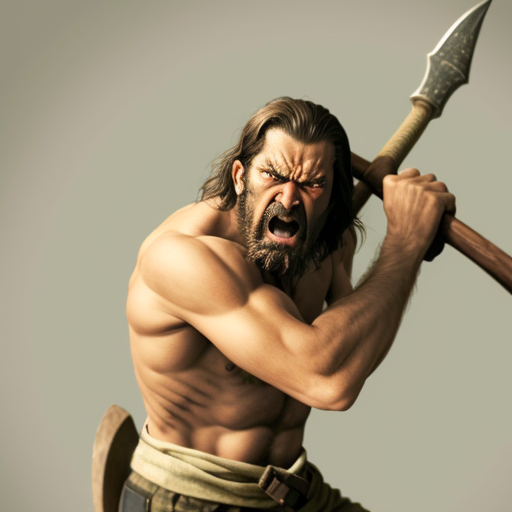
\includegraphics{an-angry-man-with-a-double-axe.png}
\end{figure}

\subsection{Descrizione Generale}\label{descrizione-generale}


Grunt è un nano robusto e massiccio, con mani grosse e callose,
testimonianza dei lunghi anni trascorsi a lavorare con materiali grezzi
nelle montagne. Indossa abiti robusti e pratici, preferendo pelli e
tessuti resistenti per sopportare le dure condizioni del mondo esterno.
Sulla schiena porta una ascia bipenne, sua arma preferita.

\begin{quote}
``Tu! Dammi altro cibo!''
\end{quote}

\subsection{Biografia}\label{biografia}


Grunt è nato e cresciuto tra le montagne a sud di Azura, con la tribù
dei Martelcuore, un gruppo di nani che ha sempre disdegnato la civiltà.
La sua infanzia è stata segnata da giorni trascorsi nelle grotte e nelle
valli nascoste tra montagne, imparando a sopravvivere grazie a un
profondo legame con la natura circostante. Grunt ha sviluppato una forza
brutale che lo ha fatto risaltare tra i suoi simili.

\subsection{Carriera}\label{carriera}


Un incontro casuale con un gruppo di avventurieri provenienti dalla
Gilda dei Protettori di Azura ha cambiato la vita di Grunt. La sua
incredibile abilità nel combattimento e la sua capacità naturale di
sopravvivenza lo hanno reso un membro apprezzato della gilda. Grunt ha
abbandonato la vita nelle montagne per unirsi alla Gilda dei Protettori
di Azura, aprendo così le porte alla scoperta di nuove terre e
avventure. Combattendo per la gilda, Grunt ha dimostrato di essere un
alleato valoroso, anche se la sua scarsa conoscenza delle città e delle
leggi lo porta spesso in situazioni comiche.

\subsection{Personalità}\label{personalituxe0}

Grunt è noto per la sua lealtà e per il suo stomaco senza fondo. La sua
natura barbarica si combina con una curiosità ingenua nei confronti
della civiltà, portandolo a imparare lentamente le stranezze della vita
in città. È un combattente determinato, pronto a proteggere i suoi
alleati con la sua forza brutale. La sua semplicità e il suo spirito
libero possono portare a momenti di comicità e imbarazzo, ma la sua
genuinità lo rende un amico fidato e un compagno di avventura pronto a
tutto, soprattutto quando viene ricompensato con un lauto pasto. Grunt è
ansioso di esplorare il mondo al di fuori delle montagne e sta appena
iniziando la sua avventura.



\section{Hartley}\label{hartley}


\begin{figure}
\centering
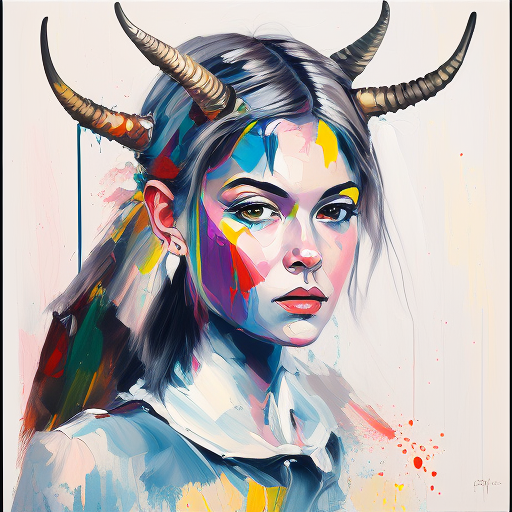
\includegraphics{Hartley_autoritratto.png}
\caption{Hartley\_autoritratto.png}
\end{figure}

Informazioni Generali

Età: 25

Anno di nascita: 1998

Paese di nascita: Kos

Razza: Tiefling

Relazioni:

Alleati:

Nemesi:

Possedimenti importanti:


\subsection{Descrizione Generale}\label{descrizione-generale}


\begin{figure}
\centering
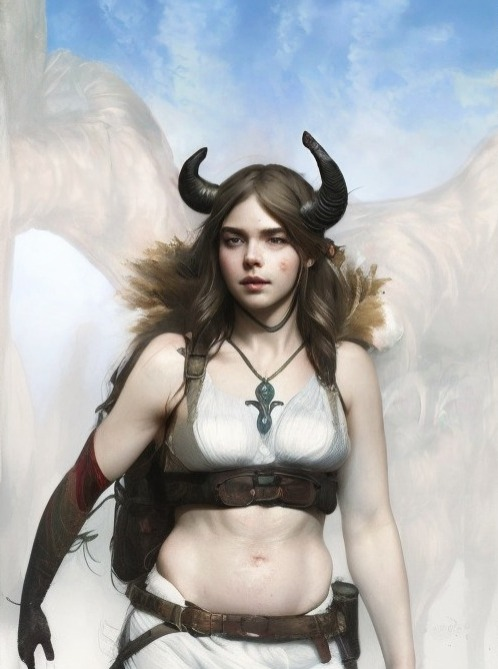
\includegraphics{Hartley.jpeg}
\caption{Hartley.jpeg}
\end{figure}

Lettera di risposta di Marpalo (Quartiermastro dei Protettori di Kos)
alla richiesta di Sitahu di inviare ad Azura un protettore adatto ad una
missione di spionaggio.

``Come mi hai chiesto, ecco tutto quello che so su Hartley Nessuno
conosce la sua vera storia, perché racconta una cosa diversa ogni volta
che qualcuno gliela chiede. A volte è scappata dall'estremo Nord a causa
delle persecuzioni contro i tiefling, altre volte è un'ex prostituta che
ha dovuto uccidere il suo pappone per conquistare la propria libertà,
altre ancora una principessa scappata dal massacro della sua famiglia
durante le rivolte popolari di chissà quale regno lontano. Non
conosciamo neanche il suo cognome, in tasca ha sempre più di un
documento pronto a testimoniare in favore delle sue molteplici
personalità. Probabilmente neanche lei si ricorda più come si chiama.
Bugiarda patologica, ma convincente, mente anche quando non c'è alcun
motivo valido per farlo. Il problema più grande è il suo modo di fare:
sempre cordiale, di buon umore, pronta ad ascoltare e a compatire.
Diresti di lei che è la tua amica più fidata, almeno fino a quando non
riesce ad ottenere da te quello di cui aveva bisogno. Di lei sappiamo
solo che si guadagnava da vivere per strada, distraendo i passanti con
giochi di prestigio e derubandoli mentre lo faceva. Alla fine dello
spettacolo le lasciavano anche qualche monetina (se non le aveva già
prese)! Col passare del tempo ha alzato il tiro, arrivando a svaligiare
le case e gli appartamenti dei cittadini più ambienti della città, fino
a quando non ha fatto il passo più lungo della gamba. Ha deciso di
introdursi nella casa di noto politico Kosentino, uno degli uomini più
influenti di Kos, con una delle case più sorvegliate della città. È
riuscita ad entrare senza fatica, e di questo le bisogna dare merito, ma
non è più uscita. Dopo essere stata catturata avrebbe potuto finire il
resto dei suoi giorni in galera, ma per sua fortuna il suo bersaglio è
anche uno dei principali benefattori della Gilda dei Protettori, e le ha
proposto di mettere le sue capacità al servizio dei bisognosi, lavorando
per la Gilda. In cambio avrebbe fatto decadere tutte le accuse che
gravavano sulla sua testa. Ancora ci chiediamo come sia possibile che le
abbia concesso una grazia del genere, probabilmente è caduto vittima dei
suoi incantesimi da manipolatrice! È stata scortata alla Gilda dalle
guardie cittadine, che hanno presidiato la nostra sede per poco più di
una settimana, poi sono sparite. Hartley da allora è con noi, anche se
adesso potrebbe scappare con il nostro equipaggiamento e spacciarsi per
una Protettrice. Si è rivelata un'ottima risorsa in più di una missione,
riesce ad a trovare una soluzione anche nelle situazioni più difficili,
e non c'è serratura che riesca a fermarla. Tuttavia si rifiuta di
combattere, non si abbassa a ``barbarie del genere'', come dice spesso.
``Le giuste parole aprono più teste di una scure'' dice anche. Spero che
queste informazioni ti possano essere utili nella scelta dei componenti
per la tua squadra. Porta i miei saluti alla tua Francine e ai piccoli
Tuo Marpalo''


\subsection{Coinvolgimenti in eventi
recenti}\label{coinvolgimenti-in-eventi-recenti}


\href{Untitled\%20Database\%20f0a0837cffd44ac7a9471133f60c97b8.csv}{Untitled
Database}

\subsection{6. Scheda personaggio}\label{scheda-personaggio}


\href{Info\%20PG\%20792973e9c98e424b8fa1da3d1c2eeac4.csv}{Info PG}

\subsubsection{Statistiche e abilità}\label{statistiche-e-abilituxe0}


\href{Abilita\%CC\%80\%207db3a6b653ad434187ea54a65d788929.csv}{Abilità}

\subsubsection{Lista magie}\label{lista-magie}


\section{Ken Nataro}\label{ken-nataro}
\section{Ken Nataro}\label{ken-nataro-1}


\begin{figure}
\centering
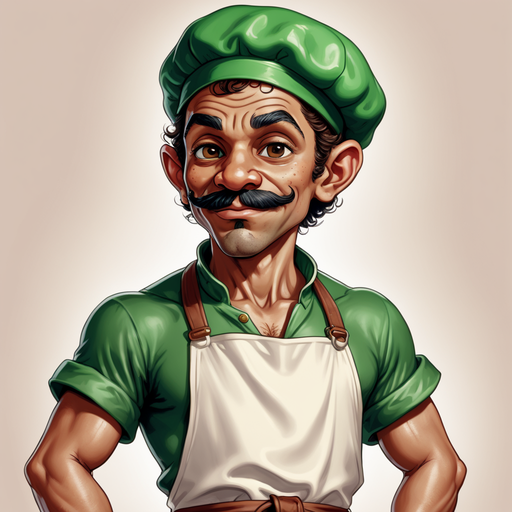
\includegraphics{create-a-digital-illustration-of-ken-nataro-a-mulatto-skinned-halfling-with-a-sturdy-physique-ken--7.png}
\caption{create-a-digital-illustration-of-ken-nataro-a-mulatto-skinned-halfling-with-a-sturdy-physique-ken--7.png}
\end{figure}

Informazioni Generali

Età: 59

Data di nascita: 20/04/1964

Luogo di nascita: Kos

Razza: Halfling

Relazioni: Sposato con Balorca

Alleati: Gilda dei protettori

Alias: U furnaru

Professione: Panettiere


\subsection{Descrizione Generale}\label{descrizione-generale}


\begin{figure}
\centering
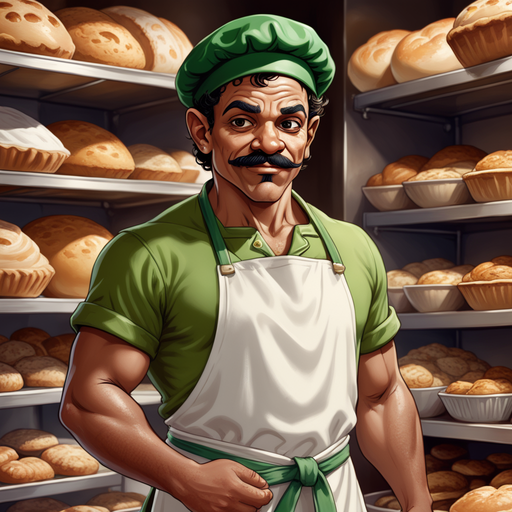
\includegraphics{create-a-digital-illustration-of-ken-nataro-a-mulatto-skinned-halfling-with-a-sturdy-physique-ken--9.png}
\caption{create-a-digital-illustration-of-ken-nataro-a-mulatto-skinned-halfling-with-a-sturdy-physique-ken--9.png}
\end{figure}

Ken Nataro è un halfling di anni con un aspetto insolito per la sua
razza. È dotato di potenti braccia muscolose, frutto di anni e anni di
duro lavoro nella sua panetteria ``da Nataro''. La sua pelle è
abbronzata dal sole e il suo viso mostra rughe di esperienza e di vita
vissuta. I suoi occhi sono vivaci e riflettono la profonda ira che
cresce in lui quando si trova di fronte all'ingiustizia.

\subsection{Biografia}\label{biografia}


\subsubsection{Infanzia}\label{infanzia}

Ken Nataro è nato in una famiglia di panettieri halfling con una
tradizione secolare di produzione del pane. Fin da piccolo, Ken mostrava
un interesse vivace per il mestiere di famiglia. Mentre i suoi coetanei
giocavano a nascondino, Ken preferiva impastare la pasta e osservare il
pane lievitare nel forno a legna. La panetteria ``da Nataro'' era il
cuore pulsante della comunità halfling di Kos, e Ken amava passare il
tempo con i suoi genitori e i suoi nonni mentre apprendeva i segreti
dell'arte della panificazione.

\subsubsection{\texorpdfstring{\textbf{Eredità della
Panetteria}}{Eredità della Panetteria}}\label{eredituxe0-della-panetteria}

All'età di anni, dopo anni di apprendistato e duro lavoro nella
panetteria di famiglia, Ken ereditò ufficialmente la gestione della
panetteria ``da Nataro'' dai suoi genitori. Questo fu un momento di
grande responsabilità, ma anche di orgoglio per Ken, che si sentiva
onorato nel portare avanti la tradizione familiare. La panetteria era
famosa in tutta Kos per il suo pane fragrante e le sue prelibatezze da
forno, che erano richieste persino dai nobili di Kos durante le
festività.

\subsubsection{\texorpdfstring{\textbf{La Lenta
Decadenza}}{La Lenta Decadenza}}\label{la-lenta-decadenza}

Nonostante il suo impegno instancabile e il desiderio di preservare la
gloria della panetteria, Ken dovette affrontare tempi difficili. I
cambiamenti nel commercio del grano e le fluttuazioni economiche in Kos
iniziarono a colpire la sua attività. La panetteria ``da Nataro'' non
era più la potenza economica di un tempo, e Ken faticava a mantenere i
livelli di produzione e a sbarcare il lunario. Questi tempi difficili
fecero emergere in lui la sua innata ira e desiderio di ristabilire
l'equilibrio nella sua vita.

\subsubsection{\texorpdfstring{Entrata ne\textbf{lla Gilda dei
Protettori}}{Entrata nella Gilda dei Protettori}}\label{entrata-nella-gilda-dei-protettori}

Per affrontare le crescenti difficoltà finanziarie e sostenere la sua
numerosa famiglia, Ken prese una decisione radicale. All'età di anni,
lasciò la gestione quotidiana della panetteria nelle mani di sua moglie,
Balorca, una mezz'orca dal cuore gentile, e decise di unirsi alla Gilda
dei Protettori. Questa decisione fu dettata dalla necessità di
guadagnare un reddito extra, ma anche dalla sua crescente ira per le
ingiustizie del mondo. Ken trasformò la sua rabbia in una forza
formidabile nel campo di battaglia, diventando un membro valoroso della
gilda. Oggi, Ken Nataro bilancia la sua vita da panettiere con le sue
nuove avventure come barbaro nella Gilda dei Protettori. La sua
dedizione alla sua famiglia, la sua passione per la panificazione e il
suo desiderio di giustizia sono i pilastri della sua vita, rendendolo un
personaggio complesso e affascinante nel mondo di Kos.

\subsection{Personalità}\label{personalituxe0}


Ken Nataro è un individuo di straordinaria forza d'animo e
determinazione. La sua personalità è caratterizzata da un profondo senso
di responsabilità e un attaccamento radicato alla sua famiglia e alla
sua tradizione. È gentile e affettuoso con i suoi dieci figli, e la sua
relazione con sua moglie, Balorca, è fondata su un amore profondo e una
profonda comprensione reciproca.

Tuttavia, sotto la superficie calma e affettuosa, alberga una fiamma di
ira ardente. Le ingiustizie del mondo, in particolare quelle che hanno
colpito la sua amata panetteria di famiglia, alimentano la sua
determinazione a fare del bene e a ristabilire l'equilibrio. Quando si
trova di fronte all'ingiustizia o alla crudeltà, questa ira si trasforma
in una forza indomabile che lo guida in battaglia, conferendo a Ken un
coraggio straordinario e una capacità di combattimento formidabile.

Ken è anche noto per la sua generosità e la sua propensione a sostenere
chi è in difficoltà, e questo lo rende un membro prezioso della Gilda
dei Protettori. È sempre pronto a tendere una mano agli amici e agli
alleati e a difendere coloro che non possono difendersi da soli. La sua
personalità complessa, con una mescolanza di gentilezza, ira e spirito
combattivo, lo rende un personaggio affascinante e un alleato fidato
nelle avventure di Kos

\subsection{Coinvolgimenti in eventi
recenti}\label{coinvolgimenti-in-eventi-recenti}


\href{Untitled\%206d32341cd290432098378da8e9e19b98.csv}{}


\section{Kit (WIP)}\label{kit-wip}


\begin{figure}
\centering

\includegraphics{No-Photo-Available-591x591-2.jpg}
\caption{No-Photo-Available-591x591-2.jpg}
\end{figure}

Informazioni Generali

Età:

Anno di nascita:

Paese di nascita:

Razza:

Relazioni:

Alleati:

Nemesi:

Possedimenti importanti:


\subsection{Descrizione Generale}\label{descrizione-generale}


\begin{figure}
\centering
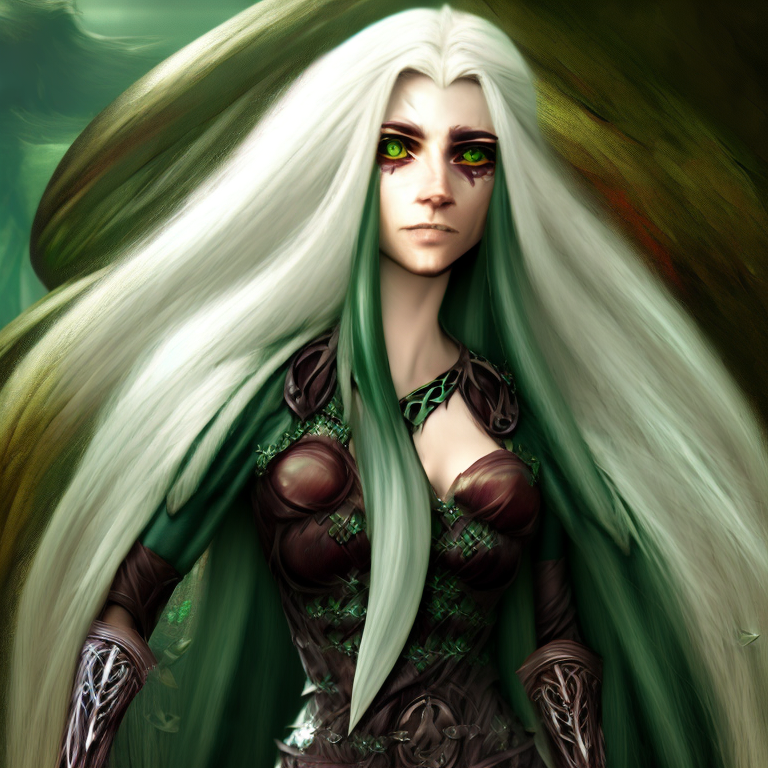
\includegraphics{full-body-portrait-of-a-beautiful-female-elf-with-long-silver-hairs-and-deep-green-eyes-fantasy-se-.png}
\caption{full-body-portrait-of-a-beautiful-female-elf-with-long-silver-hairs-and-deep-green-eyes-fantasy-se-.png}
\end{figure}

{[}Location{]} is the largest {[}location type{]} in the {[}larger
location{]} within the {[}geographic area{]} of {[}larger geographic
area{]}. {[}Location{]} neighbors {[}other location{]} to the
{[}direction{]} and {[}other location{]} to the {[}other direction{]}.
Known for being a place of {[}description{]}, {[}location{]} is home to
{[}people group{]} and the {[}organization{]}.

\begin{quote}
Citazione {[}location{]}
\end{quote}

\subsection{Biografia}\label{biografia}


The {[}people group{]} were the region's sole residents prior to the
{[}historical event{]}. {[}New people group{]} arrived in the region
around {[}year{]}.

\subsection{Carriera}\label{carriera}


The history and economic growth of {[}location{]} is tied to
{[}geographic feature{]} which is {[}location's{]} defining
characteristic.

\subsection{Personalità}\label{personalituxe0}



\section{Mortimer}\label{mortimer}


\begin{figure}
\centering
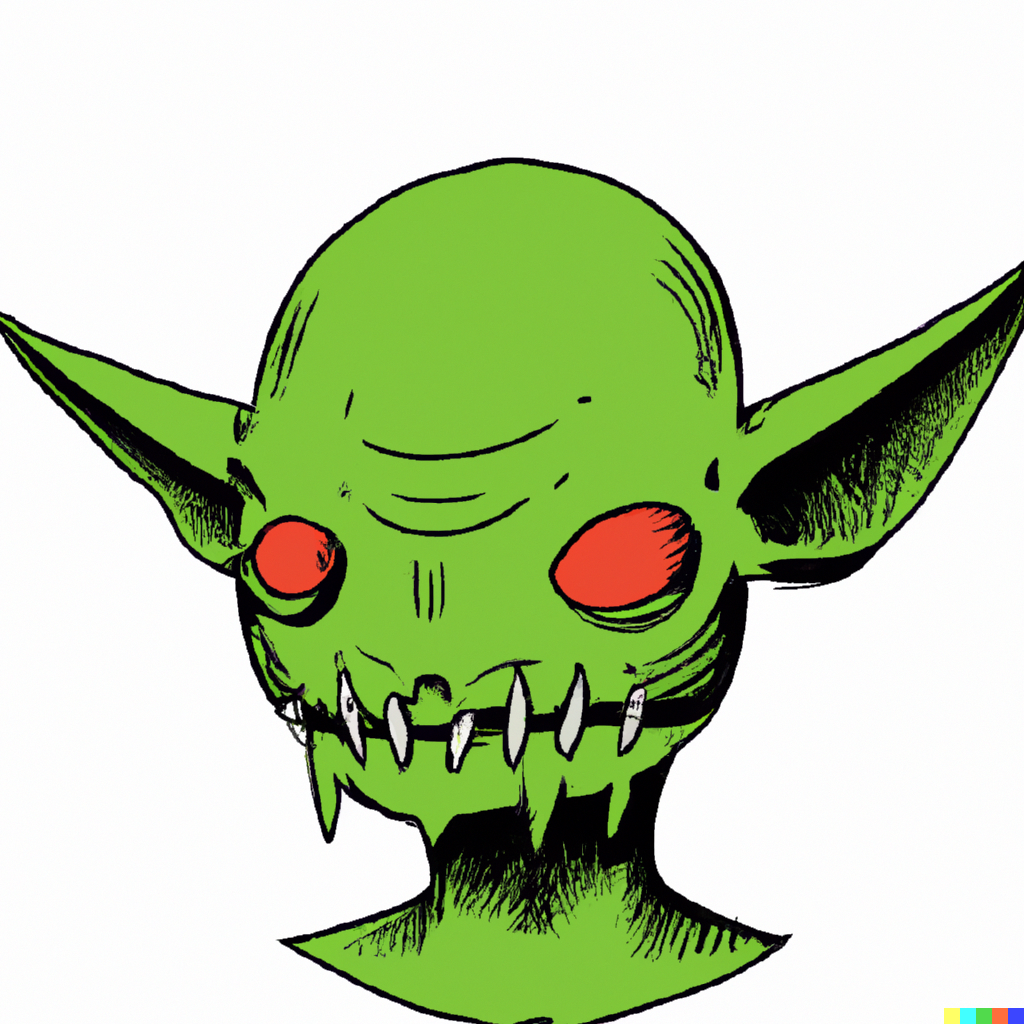
\includegraphics{Mortimer.png}
\caption{Mortimer.png}
\end{figure}

{[}Info generali{]}

Età: 12

Anno di nascita: 2011

Paese di nascita:

Razza: Goblin

Relazioni: Gilda dei Protettori

Alleati:

Nemesi:

Possedimenti importanti:


\subsection{Descrizione Generale}\label{descrizione-generale}


\begin{figure}
\centering
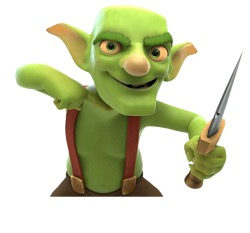
\includegraphics{Goblins_card_render.jpeg}
\caption{Goblins\_card\_render.jpeg}
\end{figure}

Un guerriero goblin con disturbo dell'attenzione.

\begin{quote}
``Voglio assaggiare quest'acqua di fogna''
\end{quote}

\subsection{Biografia}\label{biografia}


\begin{figure}
\centering
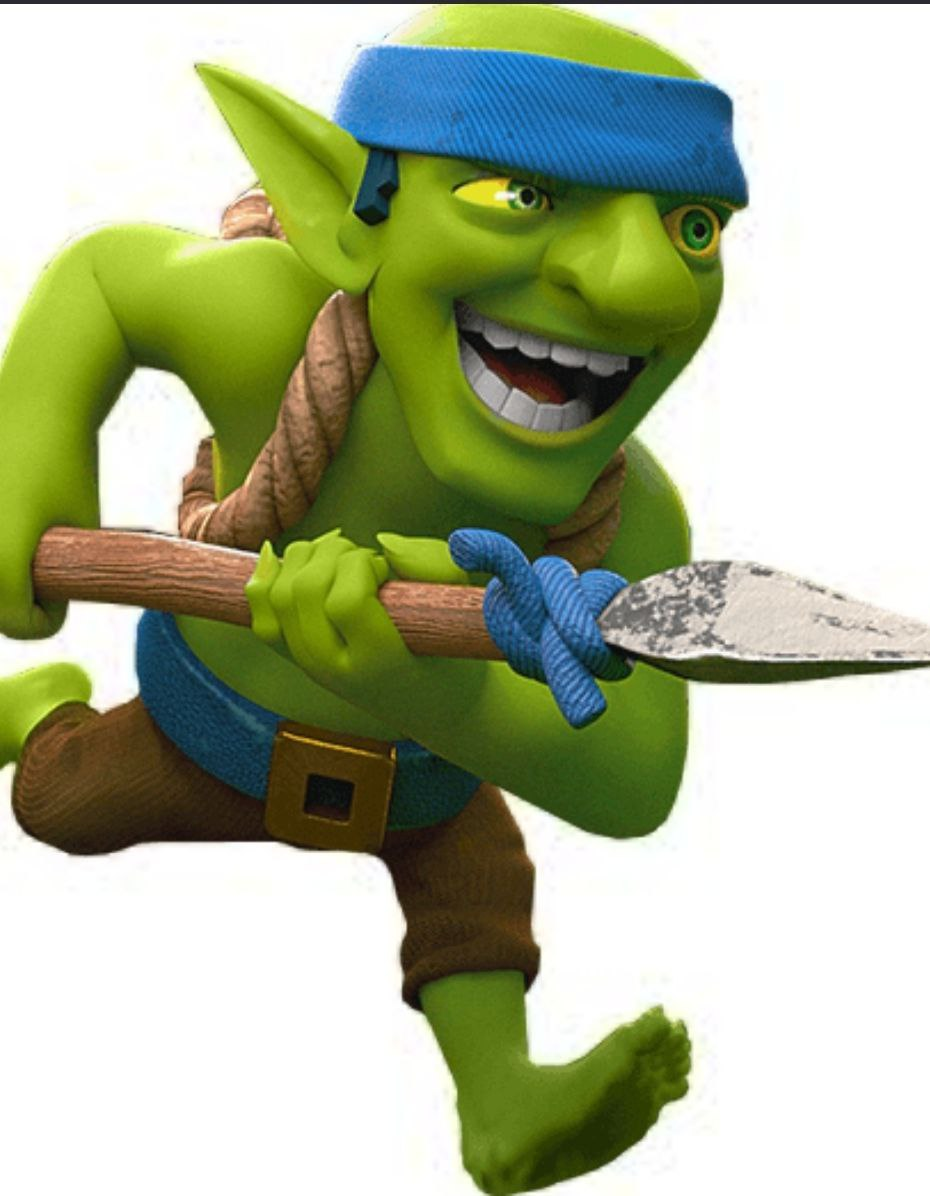
\includegraphics{2023-03-26_17.20.08.jpg}
\caption{2023-03-17.20.08.jpg}
\end{figure}

I genitori lo hanno mandato all'accademia militare con la speranza che
apprendesse disciplina e educazione, ma è scappato dopo un anno.

I genitori ancora lo cercano.

Per guadagnarsi da vivere ha scelto la strada più facile e sbagliata: il
crimine. Non ha legami con alcuna organizzazione in particolare,ma ha
dei contatti nella mala. Ogni tanto lo chiamano per dei lavori,
principalmente colpi a diligenze.

\subsection{Carriera}\label{carriera}


Nell'ultimo periodo si è affiliato alla Gilda dei Protettori della Sila
devoti a San Francesco e ai Lupi, un buon ``tetto sulla testa e una paga
decente'' a suo parere.

\subsection{Personalità}\label{personalituxe0}


Non ha ben in mente cosa sia bene e male, ma non perchè sia un goblin
(basta con gli stereotipi), viene da una famiglia per bene, gente che
gli ha dato un fior fiore di educazione\ldots{} Proprio è una testina di
cazzo.


\section{Pippo Francfrog}\label{pippo-francfrog}


\begin{figure}
\centering
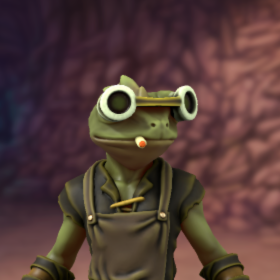
\includegraphics{Pippo_Francfrog-Token.png}
\end{figure}

\subsection{Descrizione Generale}\label{descrizione-generale}



Pippo Francfrog incarna l'incantevole fusione di una rana umanoide e la
magia dell'intrattenimento. La sua pelle iridescente rivela radici
anfibie, mentre lo sguardo intelligente brilla di carisma. Con abiti
vivaci e un sorriso contagioso, Pippo attrae l'attenzione ovunque vada.
La sua natura di artista si riflette in ogni gesto, mantenendo viva la
luce del palcoscenico anche mentre esplora nuovi orizzonti.

\begin{quote}
``Torte in faccia!''
\end{quote}

\subsection{Biografia}\label{biografia}


\subsubsection{Infanzia e le OriginiMistiche}\label{infanzia-e-le-origini-mistiche}
Pippo Francfrog vide la luce grazie a un incantesimo complesso e ardito
lanciato dal mago Lasalmadi Mikebongiorno. La sua creazione era un
tentativo di fondere la magia con il mondo dell'intrattenimento,
producendo così una creatura unica nel suo genere. Sin dalla sua
nascita, Pippo ha portato con sé un legame con la magia che avrebbe
influenzato il corso della sua vita.

\subsubsection{Esordi in ``Il Bagaglione''}
I primi passi di Pippo nel mondo dell'intrattenimento li compì entrando
a far parte dello spettacolo itinerante de ``Il Bagaglione''. Qui, Pippo
fu introdotto all'arte dell'intrattenimento e imparò i segreti
dell'interazione con il pubblico. Le sue performance coinvolgenti e
innovative catturarono l'attenzione di tutti coloro che ebbero la
fortuna di assistere ai suoi numeri.

\subsubsection{Richiamo della Magia e il Percorso come Artificiere}
Mentre il suo talento nel campo dell'intrattenimento si faceva sempre
più evidente, la sua connessione con la magia iniziò a emergere in modo
più preponderante. Sentendo il richiamo della magia dentro di sé, Pippo
intraprese un nuovo cammino come artificiere. La sua abilità nel creare
oggetti incantati e invenzioni uniche gli permise di esprimere la sua
creatività in modi mai sperimentati prima.

\subsubsection{Unione Fraterna con Pippo Baudog}
Le avventure di Pippo non furono mai solitarie. Insieme a suo fratello
Pippo Baudog, un cane antropomorfo con il medesimo retaggio magico,
intraprese molte imprese. La loro partnership rappresentava l'armoniosa
fusione tra intrattenimento e abilità magica, dimostrando il valore
dell'affetto fraterno nel raggiungimento dei traguardi.

\subsubsection{Eredità e Impatto}
La vita di Pippo Francfrog è rimasta una testimonianza dell'incrocio tra
il mondo della magia e dell'intrattenimento. La sua biografia incarna la
perseveranza nella ricerca della propria passione, nonostante le diverse
sfaccettature della sua identità. La sua eredità continua a ispirare
coloro che cercano di fondere passioni divergenti, aprendo la strada a
un mondo di meraviglia, sorpresa e collaborazione.

\subsection{Carriera}\label{carriera}


La carriera di Pippo Francfrog è stata un connubio straordinario tra
magia e intrattenimento. Dopo esordi di successo con lo spettacolo
itinerante de ``Il Bagaglione'', Pippo ha seguito il richiamo della
magia e si è dedicato all'artigianato magico come artificiere.
Nonostante questo cambiamento di percorso, non ha mai dimenticato le sue
radici da intrattenitore, portando sempre con sé il desiderio di
incantare e stupire il pubblico. Collaborando spesso con suo fratello,
Pippo Baudog, ha dimostrato come la fusione di talento e creatività
possa creare un'esperienza unica e indimenticabile per chiunque lo
incontri. La sua carriera è un esempio di come diverse passioni possano
coesistere e arricchirsi a vicenda, creando un mondo di meraviglia e
sorpresa.

\subsection{Personalità}\label{personalituxe0}


La personalità di Pippo Francfrog è un affascinante mix di carisma,
curiosità e creatività. È un individuo straordinariamente affabile, con
un sorriso contagioso e uno sguardo che riflette un'intelligenza
brillante. La sua natura di intrattenitore è evidente in ogni aspetto
della sua vita, portando con sé l'abilità di incantare e stupire
chiunque incontri. La sua curiosità insaziabile lo spinge a esplorare
nuovi orizzonti, sia nell'arte dello spettacolo che nell'artigianato
magico. Tuttavia, il suo cuore rimane fedele al desiderio di portare
gioia e meraviglia al pubblico, e questa passione è il motore che guida
ogni sua azione. La sua personalità è un richiamo costante alla magia
della creatività e all'importanza di diffondere la gioia attraverso
l'arte e lo spettacolo.


\section{Sabaku no Darude}\label{sabaku-no-darude}


\begin{figure}
\centering
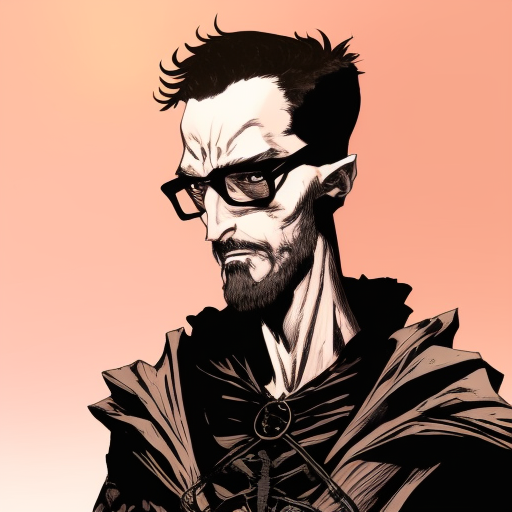
\includegraphics{blkmndy_fantasy_character_with_a_hooded_cape_with_a_beard_with_glasses.png}
\end{figure}

\subsection{Descrizione Generale}\label{descrizione-generale}



Sabaku no Darude è un mezzelfo nato in una landa desertica del
continente. Ha una combinazione di tratti sia umani che elfici, con una
pelle leggermente scura e capelli castani mossi. I suoi occhi, di un
colore ambrato brillante, riflettono la sua passione interiore.

\begin{quote}
``Per chi conosce la Lore. Per chi la sta scoprendo. Per chi la
scoprirà'' - Sabaku no Darude
\end{quote}

\subsection{Biografia}\label{biografia}


Sabaku no Darude è cresciuto in una landa desertica dopo la morte dei
suoi genitori mercenari quando aveva solo 5 anni. Ha vissuto con il suo
saggio nonno materno, un elfo che gli ha trasmesso l'amore per la musica
e l'arte. Grazie alle storie epiche e alle ballate antiche che ha
ascoltato, Darude ha sviluppato un profondo desiderio di condividerle
con tutte le razze del mondo.

\subsection{Carriera}\label{carriera}


Per realizzare il suo desiderio di diffondere conoscenza e creare un
legame tra le persone, Darude ha intrapreso un viaggio come bardo
itinerante. Durante i suoi viaggi, esplora nuovi luoghi, impara le
storie locali e interagisce con le diverse culture e razze. Durante
queste esperienze, scrive di sé stesso e degli avvenimenti che gli
accadono intorno, creando un diario di viaggio personale.

Darude si esibisce in vari luoghi, dalle taverne dei villaggi alle corti
dei re, utilizzando la sua abilità musicale e le sue doti di narratore
per coinvolgere il pubblico. La sua musica tocca le corde dell'anima e
le sue storie ispirano gli ascoltatori a guardare al di là delle
differenze e a trovare un terreno comune.

\subsection{Personalità}\label{personalituxe0}


Darude è una persona gentile e appassionata, con una grande curiosità e
apertura mentale. È rispettoso delle tradizioni locali e cerca sempre di
creare comprensione reciproca tra le diverse razze. La sua passione per
la musica e le storie è contagiosa e porta gioia ovunque vada. Ha
un'anima creativa e un cuore generoso, e cerca di utilizzare le sue
abilità per rendere il mondo un posto migliore.


\section{Stalag Might}\label{stalag-might}


\begin{figure}
\centering
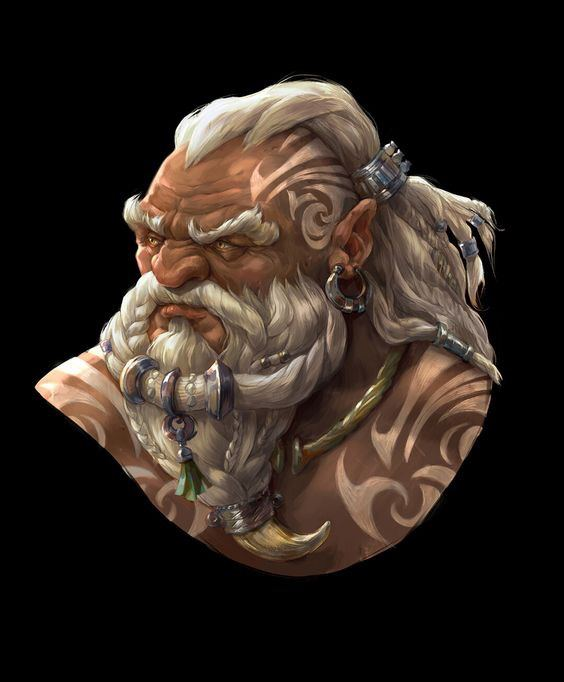
\includegraphics{2023-09-17_22.34.48.jpg}
\end{figure}

\subsection{Descrizione Generale}\label{descrizione-generale}


Stalag Might è un nano druido le cui origini sono radicate nelle
profondità di una montagna antica conosciuta come ``Lunacrest''. La sua
storia è intrecciata con il mistero di questa montagna, dove le energie
dell'antica luna scorrono nelle vene stesse della terra. Conosciuto tra
i druidi come il ``Bambino delle Rocce'', Stalag ha sempre mostrato una
connessione innata con le pietre e una passione per la geologia.

\begin{quote}
``Bella questa roccia''
\end{quote}

\subsection{Biografia}\label{biografia}


\subsubsection{Infanzia}\label{infanzia}


Stalag Might nacque nelle viscere di Lunacrest, portando con sé una
strana formazione rocciosa sulla mano sinistra, simile alle maestose
montagne circostanti. Questo segno innato attirò l'attenzione dei suoi
genitori, che lo condussero alla congrega dei druidi del Circolo della
Luna quando era ancora un neonato. Il giovane nano cresceva, diventando
noto tra i druidi come il ``Bambino delle Rocce''. La sua forza fisica e
la sua passione per la geologia lo resero un apprendista straordinario.

\subsubsection{Adolescenza}\label{adolescenza}


Durante gli anni della sua formazione, Stalag sviluppò un profondo
interesse per la metamorfosi, una delle abilità centrali dei druidi del
Circolo della Luna. A differenza dei suoi compagni, prediligeva
trasformarsi in piccoli animali, come topi, talpe e lucertole, per
esplorare fessure e cavità inaccessibili. Questa abilità gli consentiva
di scoprire gemme nascoste e segreti geologici, e raccontava avventure
vissute attraverso gli occhi di un piccolo animale.

\subsubsection{Età Adulta}\label{etuxe0-adulta}


Durnan Crystalbeard, il suo anziano maestro druido, riconoscendo il
talento e la dedizione di Stalag, gli regalò un geode speciale quando il
giovane nano compì sedici anni. Questo geode, inciso con simboli
druidici, divenne sia un focus per la sua magia che un santuario per
campioni di rocce e minerali rari. Dopo aver completato la sua
formazione con la congrega, Stalag sentì il richiamo dell'esplorazione e
del desiderio di scoprire montagne e formazioni rocciose leggendarie,
alla ricerca in particolare della pietra leggendaria nota come ``Il
Cuore della Luna''.

\subsection{Personalità}\label{personalituxe0}


Stalag Might è noto per la sua mente curiosa e la passione incrollabile
per la geologia. È un individuo tranquillo ma osservatore, sempre
desideroso di ascoltare le storie delle pietre e dei minerali che
incontra lungo il suo cammino. La sua connessione con la natura e il
mondo sotterraneo lo rende rispettoso nei confronti dell'ambiente
circostante.

Inoltre, la sua abilità unica di trasformarsi in creature più piccole
gli conferisce una prospettiva unica sulla vita e sull'esplorazione.
Stalag è affezionato ai suoi compagni druidi e considera ogni avventura
come un'opportunità per arricchire la sua comprensione delle meraviglie
naturali del mondo.

Stalag Might è guidato da una doppia missione: la sete di conoscenza
geologica e la ricerca dell'enigmatica ``Pietra della Luna''. Questo
equilibrio tra scienza e magia guida le sue azioni mentre viaggia
attraverso il mondo, pronta a esplorare e a svelare i segreti che
attendono sotto le rocce e nelle profondità della terra.




\end{document}